\documentclass[conference]{IEEEtran}
\usepackage{booktabs}
\usepackage[hyphens]{url}
\usepackage[usenames,dvipsnames]{color}
\usepackage{comment}
\usepackage{float}
\usepackage{lipsum}
\usepackage{pifont}
 \usepackage[english]{babel}
\usepackage{array}
\usepackage{multirow}
\usepackage{amssymb}
\usepackage{amsthm}
\usepackage{amsmath}
\usepackage[normalem]{ulem}
\usepackage{xspace}
\usepackage{datetime}
\usepackage{hyperref}


% *** GRAPHICS RELATED PACKAGES ***
%
\usepackage[pdftex]{graphicx}
% declare the path(s) where your graphic files are
\graphicspath{{./images/}}
% and their extensions so you won't have to specify these with
% every instance of \includegraphics
\DeclareGraphicsExtensions{.pdf,.jpeg,.png}

\usepackage{etoolbox}
\makeatletter
\patchcmd{\@makecaption}
  {\scshape}
  {}
  {}
  {}
\makeatother

\hyphenation{WEB-rick op-tical net-works semi-conduc-tor}
\newcommand{\CRASH}{{\sc \{CrashSim\}}\xspace}
\hypersetup{%
%  pdftitle = {\CRASH: Catching the Unexpected},
  pdftitle = {Charting a Course Through Uncertain Environments: SEA Uses Past Problems to Avoid Future Failures}
  pdfkeywords = {},
  pdfauthor = { Names removed for anonymous submission},
  bookmarksnumbered,
  bookmarksopen=true,
  colorlinks=true,
  urlcolor=[rgb]{.35,0,0},
  linkcolor=[rgb]{.35,0,0},
  citecolor=[rgb]{.35,0,0},
  pdfstartview={FitH},
}

\usepackage{ifthen}
\usepackage[normalem]{ulem} % for \sout
\usepackage{xcolor}
\let\lneq\undefined  % removes amssymb conflict with some packages
\usepackage{amssymb}
\newcommand{\ra}{$\rightarrow$}
\newboolean{showedits}
\setboolean{showedits}{true} % toggle to show or hide edits
\ifthenelse{\boolean{showedits}}
{
	\newcommand{\ugh}[1]{\textcolor{red}{\uwave{#1}}} % please rephrase
	\newcommand{\ins}[1]{\textcolor{blue}{\uline{#1}}} % please insert
	\newcommand{\del}[1]{\textcolor{red}{\sout{#1}}} % please delete
	\newcommand{\chg}[2]{\textcolor{red}{\sout{#1}}{\ra}\textcolor{blue}{\uline{#2}}} % please change
}{
	\newcommand{\ugh}[1]{#1} % please rephrase
	\newcommand{\ins}[1]{#1} % please insert
	\newcommand{\del}[1]{} % please delete
	\newcommand{\chg}[2]{#2}
}

\newboolean{showcomments}
%\setboolean{showcomments}{true}
\setboolean{showcomments}{true}
\newcommand{\id}[1]{$-$Id: scgPaper.tex 32478 2010-04-29 09:11:32Z oscar $-$}
\newcommand{\yellowbox}[1]{\fcolorbox{gray}{yellow}{\bfseries\sffamily\scriptsize#1}}
\newcommand{\triangles}[1]{{\sf\small$\blacktriangleright$\textit{#1}$\blacktriangleleft$}}
\ifthenelse{\boolean{showcomments}}
%{\newcommand{\nb}[2]{{\yellowbox{#1}\triangles{#2}}}
{\newcommand{\nbc}[3]{
 {\colorbox{#3}{\bfseries\sffamily\scriptsize\textcolor{white}{#1}}}
 {\textcolor{#3}{\sf\small$\blacktriangleright$\textit{#2}$\blacktriangleleft$}}}
 \newcommand{\version}{\emph{\scriptsize\id}}}
{\newcommand{\nbc}[3]{}
 \renewcommand{\ugh}[1]{#1} % please rephrase
 \renewcommand{\ins}[1]{#1} % please insert
 \renewcommand{\del}[1]{} % please delete
 \renewcommand{\chg}[2]{#2} % please change
 \newcommand{\version}{}}
\newcommand{\nb}[2]{\nbc{#1}{#2}{orange}}

\definecolor{jccolor}{rgb}{0.2,0.4,0.6}
\definecolor{pmcolor}{rgb}{0.8,0.6,0.1}
\definecolor{clcolour}{rgb}{0.5,0.7,0.9}
\newcommand\cappos[1]{\nbc{JC}{#1}{jccolor}}
\newcommand\preston[1]{\nbc{PM}{#1}{pmcolor}}
\usepackage{wasysym}


\newcommand{\tickmark}{\ding{51}}
\newcommand{\xmark}{\ding{55}}

\begin{document}

\title{Charting a Course Through Uncertain Environments: SEA Uses Past Problems to Avoid Future Failures}

% author names and affiliations
% use a multiple column layout for up to three different
% affiliations
%\author{\IEEEauthorblockN{Michael Shell}
%\IEEEauthorblockA{School of Electrical and\\Computer Engineering\\
%Georgia Institute of Technology\\
%Atlanta, Georgia 30332--0250\\
%Email: http://www.michaelshell.org/contact.html}
%\and
%\IEEEauthorblockN{Homer Simpson}
%\IEEEauthorblockA{Twentieth Century Fox\\
%Springfield, USA\\
%Email: homer@thesimpsons.com}
%\and
%\IEEEauthorblockN{James Kirk\\ and Montgomery Scott}
%\IEEEauthorblockA{Starfleet Academy\\
%San Francisco, California 96678-2391\\
%Telephone: (800) 555--1212\\
%Fax: (888) 555--1212}}

\maketitle
\thispagestyle{plain}
\pagestyle{plain}

\begin{abstract}

A common problem for developers
is applications exhibiting
new bugs \textit{after} deployment.
Many of these bugs
can be traced to
unexpected network,
operating system,
and file system
differences that cause
program executions that were successful in a
development environment to fail once deployed.
Preventing these bugs is difficult because
it is impractical to test an application
in every environment.
Enter Simulating Environmental Anomalies (SEA),
a technique that utilizes evidence
of one application's failure
in a given environment
to generate tests
that can be applied to \textit{other} applications,
to see whether they suffer from analogous faults.
In SEA, models of unusual properties extracted
from interactions between an application, $A$,
and its environment guide simulations
of another application, $B$, running
in the anomalous environment.
This reveals faults $B$
may experience in this environment
without the expense of deployment.
By accumulating these anomalies,
applications can be tested against
an increasing set of problematic conditions.
We implemented a tool called CrashSimulator, which uses SEA,
and evaluated it against Linux applications
selected from coreutils and the Debian popularity contest.
Our tests found a total of 63 bugs
in 31 applications
with effects including hangs,
crashes,
data loss,
and remote denial of service conditions.

\end{abstract}

\section{Introduction}
\label{SEC:introduction}
\textit{No Battle Plan Survives Contact With the Enemy --- Helmuth von Moltke}

No matter how well an application is tested before being released, new bugs
always seem to be found after deployment.  One reason for this situation
is that applications run in a diverse set of
different deployment \emph{environments}, - and often
across different operating systems, and network types,
each of which can introduce new flaws~\cite{LinuxGlibcChanges}.
In addition, file
systems can exhibit subtle but critical
differences~\cite{EXT4Layout, AppleHFS}, and while differences in network
behavior can
be substantial, even if the network type or even the
adapter are identical~\cite{vbox}. These environmental differences greatly
exacerbate the chance of ensuring that an application will function
correctly when deployed.

This complicates the work of application developers who, according to a
recent survey conducted by ClusterHQ~\cite{ClusterHQSurvey},
spend a significant portion of their time
debugging errors that only appear in production.
Participants in this survey cited the inability to recreate
production environments for
testing as the main reason why bugs are not discovered earlier.
Even if an
enormous developer effort is put forward, it may be insufficient
to uncover these bugs
before deployment.  Microsoft employs thousands of engineers with nearly a
1:1 ratio of testers to developers~\cite{Page2009}.
Yet, recent Windows Update released in response
to the Spectre Intel CPU vulnerability resulted in machines with certain
hardware configurations were rendered unbootable~\cite{kb4056892}.  Even
specialized ``Write-Once, Run Anywhere'' environments that attempt to hide
these environmental differences, such as the Java Runtime Environment, are
not perfect, leading them to be rechristened ``Write-Once, Debug
Everywhere''~\cite{WODE}.

In this paper, we introduce {\em CrashSimulator}\footnote{ Our approach is
loosely inspired by flight simulators, which test pilot aptitude under a
variety of rare, adverse scenarios (water landings, engine failures, etc.)
before the pilots are certified to work in practice.}, a testing approach
and tool that can test an application as though it is running in a large
number of diverse environments likely to cause crashes.  It is not feasible
to test all possible environments, so an important consideration is how to
choose which environments to test.  These environments can be chosen by
identifying situations that caused environmental bugs in other applications
and then testing for them systematically.  Selecting situations in this way
means that an environmental bug that is detected in one application can be
detected by CrashSimulator in other applications.  This merely requires
CrashSimulator be configured to identify the environmental bug in question.
Once this is done, any application can be tested for the bug using
CrashSimulator with no added effort.  CrashSimulator can be configured to
test a suite of bugs accumulated from a set of applications running in a
variety of environments.  This is somewhat analogous to CrashSimulator
automatically creating unit tests for all environments in which an
application could run.  Each of these ``tests'' consists of rules for
mutating system call behavior to give the application the illusion that it
is executing in an anomalous environment and rules for determining whether
or not the application responds appropriately.  Because these rules can be
applied to many applications that may be prone to mishandling the anomalous
environment in question, prior knowledge gathered from past deployment
experiences can be used to more thoroughly work out a new application so
that it can handle the challenges of its target environments correctly.

CrashSimulator's technique for performing this testing procedure is based
on the insight that environmental anomalies can be represented as anomalies
in results and side effects of the system calls an application makes.
CrashSimulator tests an application by exposing it to these anomalous
conditions during the course of execution and evaluating the application's
response to them.  The details of this exposure are configured by taking a
system call trace of the application under normal conditions and modifying
it such that the anomalous conditions are represented.  CrashSimulator uses
these modified system call traces to control a replay execution of the
application in which these conditions will be encountered.

In the course of this work we built a proof of concept version of
CrashSimulator's technique that was able to find bugs, both known and
unknown, in popular Linux applications as ranked by Debian's popularity
contest~\cite{DebPopCon}.  These bugs were found by exposing the
applications to environmental conditions that simulate unusual file system
configurations, file types, and network delays.  When the applications in
question were actually exposed to these conditions a variety of failures
including hangs, crashes, and filesystem damage occurred.  In total, 84
bugs were identified.

In addition to these quantitative results, this paper presents the results
of a user study conducted with the goal of determining how CrashSimulator
performs in the hands of developers as they test real world applications.
This study involved ZZZ participants consisting of Master's computer
science students with varying backgrounds and specializations.  These
participants were asked to test existing popular applications (as ranked by
Debian's Popularity Contest) using CrashSimulator, AFL, and Mutiny.  This
survey yielded results in the form of numbers of bugs identified and
qualitative results about the tools' user experience through surveys.
These results show that developers are able to find new bugs with
CrashSimulator, many of which would not have been found with the other
tools due to its unique testing approach.  Additionally, survey
participants report that CrashSimulator allows them to find bugs they would
not have been about to find otherwise due to a self-reported lack of
experience with operating systems concepts.

With both sets of result in mind, the main contributions in this work are
as follows:

\begin{enumerate}

\item{It proves the importance of the interaction between an application
and its environment in creating potential flaws upon deployment.}

\item{It proposes the idea that by manipulating these interactions through
the use of system calls, the responses of an application to any given
environment can be accurately simulated without an actual
deployment to that environment.}

\item{It offers an approach for encoding an appropriate flow of
interactions between an application and its environment as a model that
can be later used to check for correct behavior.}

\item{It shows that CrashSimulator allows these developers to find real
bugs in real applications.}

\item{It provides proof that CrashSimulator compares favorably against
similar automated testing tools in the number and type of bugs found.}

\item{It submits favorable opinion results taken from study participant
survey data.}

\end{enumerate}

\section{what is an Environment?}
\label{SEC:background}

It is important
to have a clear understanding
of what constitutes an application's environment
in order to see how it can contribute to the presence of bugs.
An application's environment consists of
all of the components an application depends upon
that its developers do not control.
In practice, this is everything other than the code and data packaged
within the application itself.
Typically testers
focus on explicit inputs to the application
and overlook the implicit inputs
coming from these uncontrolled components.
Anything external to the application can be
configured in unexpected ways.
For example, library search rules can result in default system libraries
being loaded instead of
the versions deployed alongside the application.
These external resources can be thought of as
providing implicit inputs to the program that affect its flow of execution.
An investigation of bug reports has shown that environmental bugs in the
following categories have been found in major applications.

\begin{itemize}

\item {\bf Operating Systems.} Differences in the way operating systems
implement system calls can influence the behavior of applications.  For
example, on Linux it is possible to remove an open file, yet this is not
allowed on Windows systems~\cite{UnlinkStandard}.  An application
written without this difference in mind could fail if it relies on one
implementation or the other.

\item {\bf File Systems.}  The exact file system used will also have a
substantial impact on the behavior of a system, independent of the
operating system.  The popular Ext4 file system on Linux is case sensitive,
so that ``a'' and ``A'' are different files,
while in OS X's HFS+ file system
those file names would refer to the same file.
File systems can have varying limits or behaviors for other items as well,
including file name length (popularized due to the 8.3 limitations of the
FAT file system), maximum file length, number of directory entries, or
depth
of directories supported, all of which can lead to errors when programs
do not account for these variations~\cite{EXT4Layout, AppleHFS}.

\item {\bf Network.} Both local and remote network nodes
can have specific characteristics that could influence the behavior of an
application.
For example, POSIX operating
systems support the notion of limiting the kernel buffer set aside for a
socket.  However, many other popular operating
systems (Windows, Linux, and Mac)
implement this quite differently.
If a UDP datagram
larger than the specified buffer size is received by a Linux system,
it will be dropped.
Windows,
however,
will receive these datagrams,
but it will influence data retrieval.
Any system calls that retrieve data from the buffer in which
datagrams are
stored will only return a number of bytes less than or equal to the
buffer size at one time~\cite{Zhuang_NSDI_2014}.

\item {\bf Processor.}  The processor used can also influence the
behavior of an application.  This is very frequently
evidenced through the variety of different floating point behaviors a
processor may exhibit~\cite{ArbitraryPrecision}.
In addition, bugs are fairly common
in processors and will cause variances, as will
differences in interpreting
how to execute complex instructions~\cite{Microarch}.

\end{itemize}

In this work, we chose to focus on operating system,
file system, and network
environmental issues.
These issues are
readily visible in data returned
by the system calls
an application makes.
We took advantage of this in our implementation of SEA as CrashSimulator by
intercepting and manipulating system call results.
As we will discuss, this allowed us to strike a good medium between a
higher level approach such has hooking library functions and a lower level
approach like directly altering memory values.
In our evaluation we take a deeper look at anomalies from
these three categories in order to assess the technique's effectiveness.
We do not consider processor-based environmental differences as bugs related to those are being handled by other
work~\cite{Alglave:2018:FSC:3173162.3177156}.

\section{Defining and Applying the AES Technique}
\label{SEC:approach}

\begin{figure}[t]
  \center{}
  \fbox{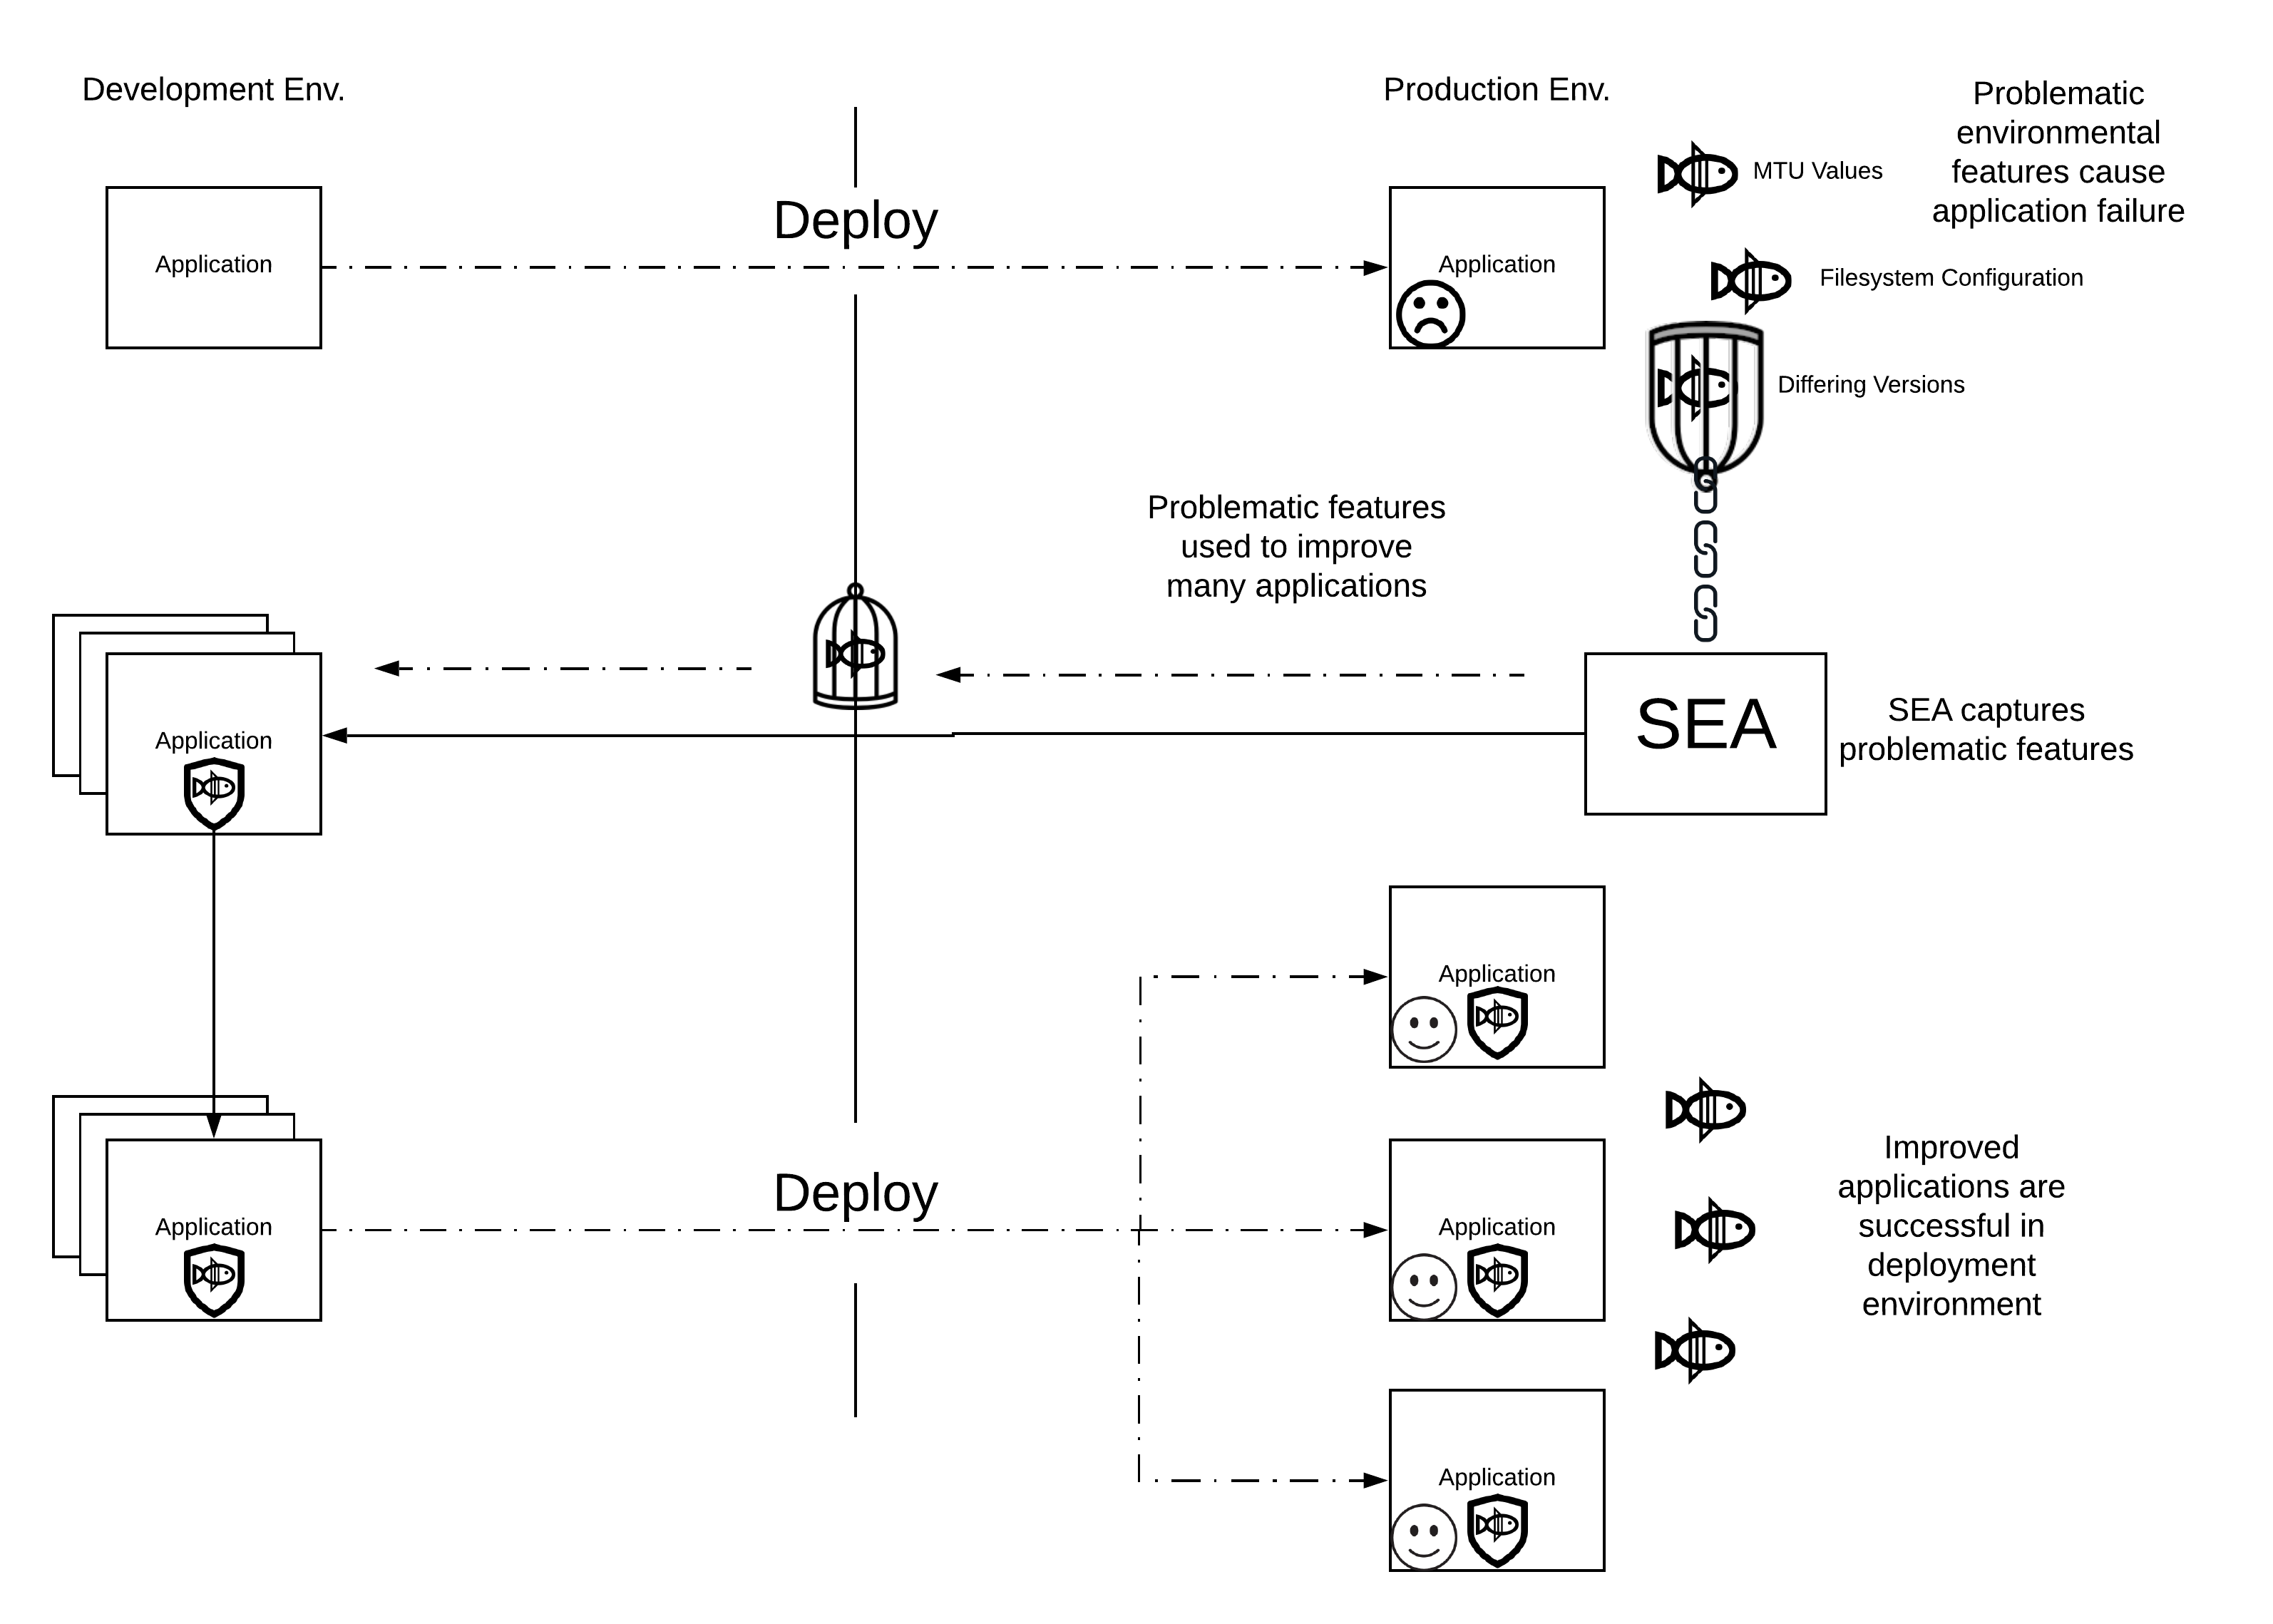
\includegraphics[scale=.37]{images/approach}}
  \caption{Diagram illustrating CrashSimulator's approach to identifying
    bugs by simulating anomalous condtions}
  \label{figure:approach}
\end{figure}

\begin{figure*}[t]
  \center{}
  \fbox{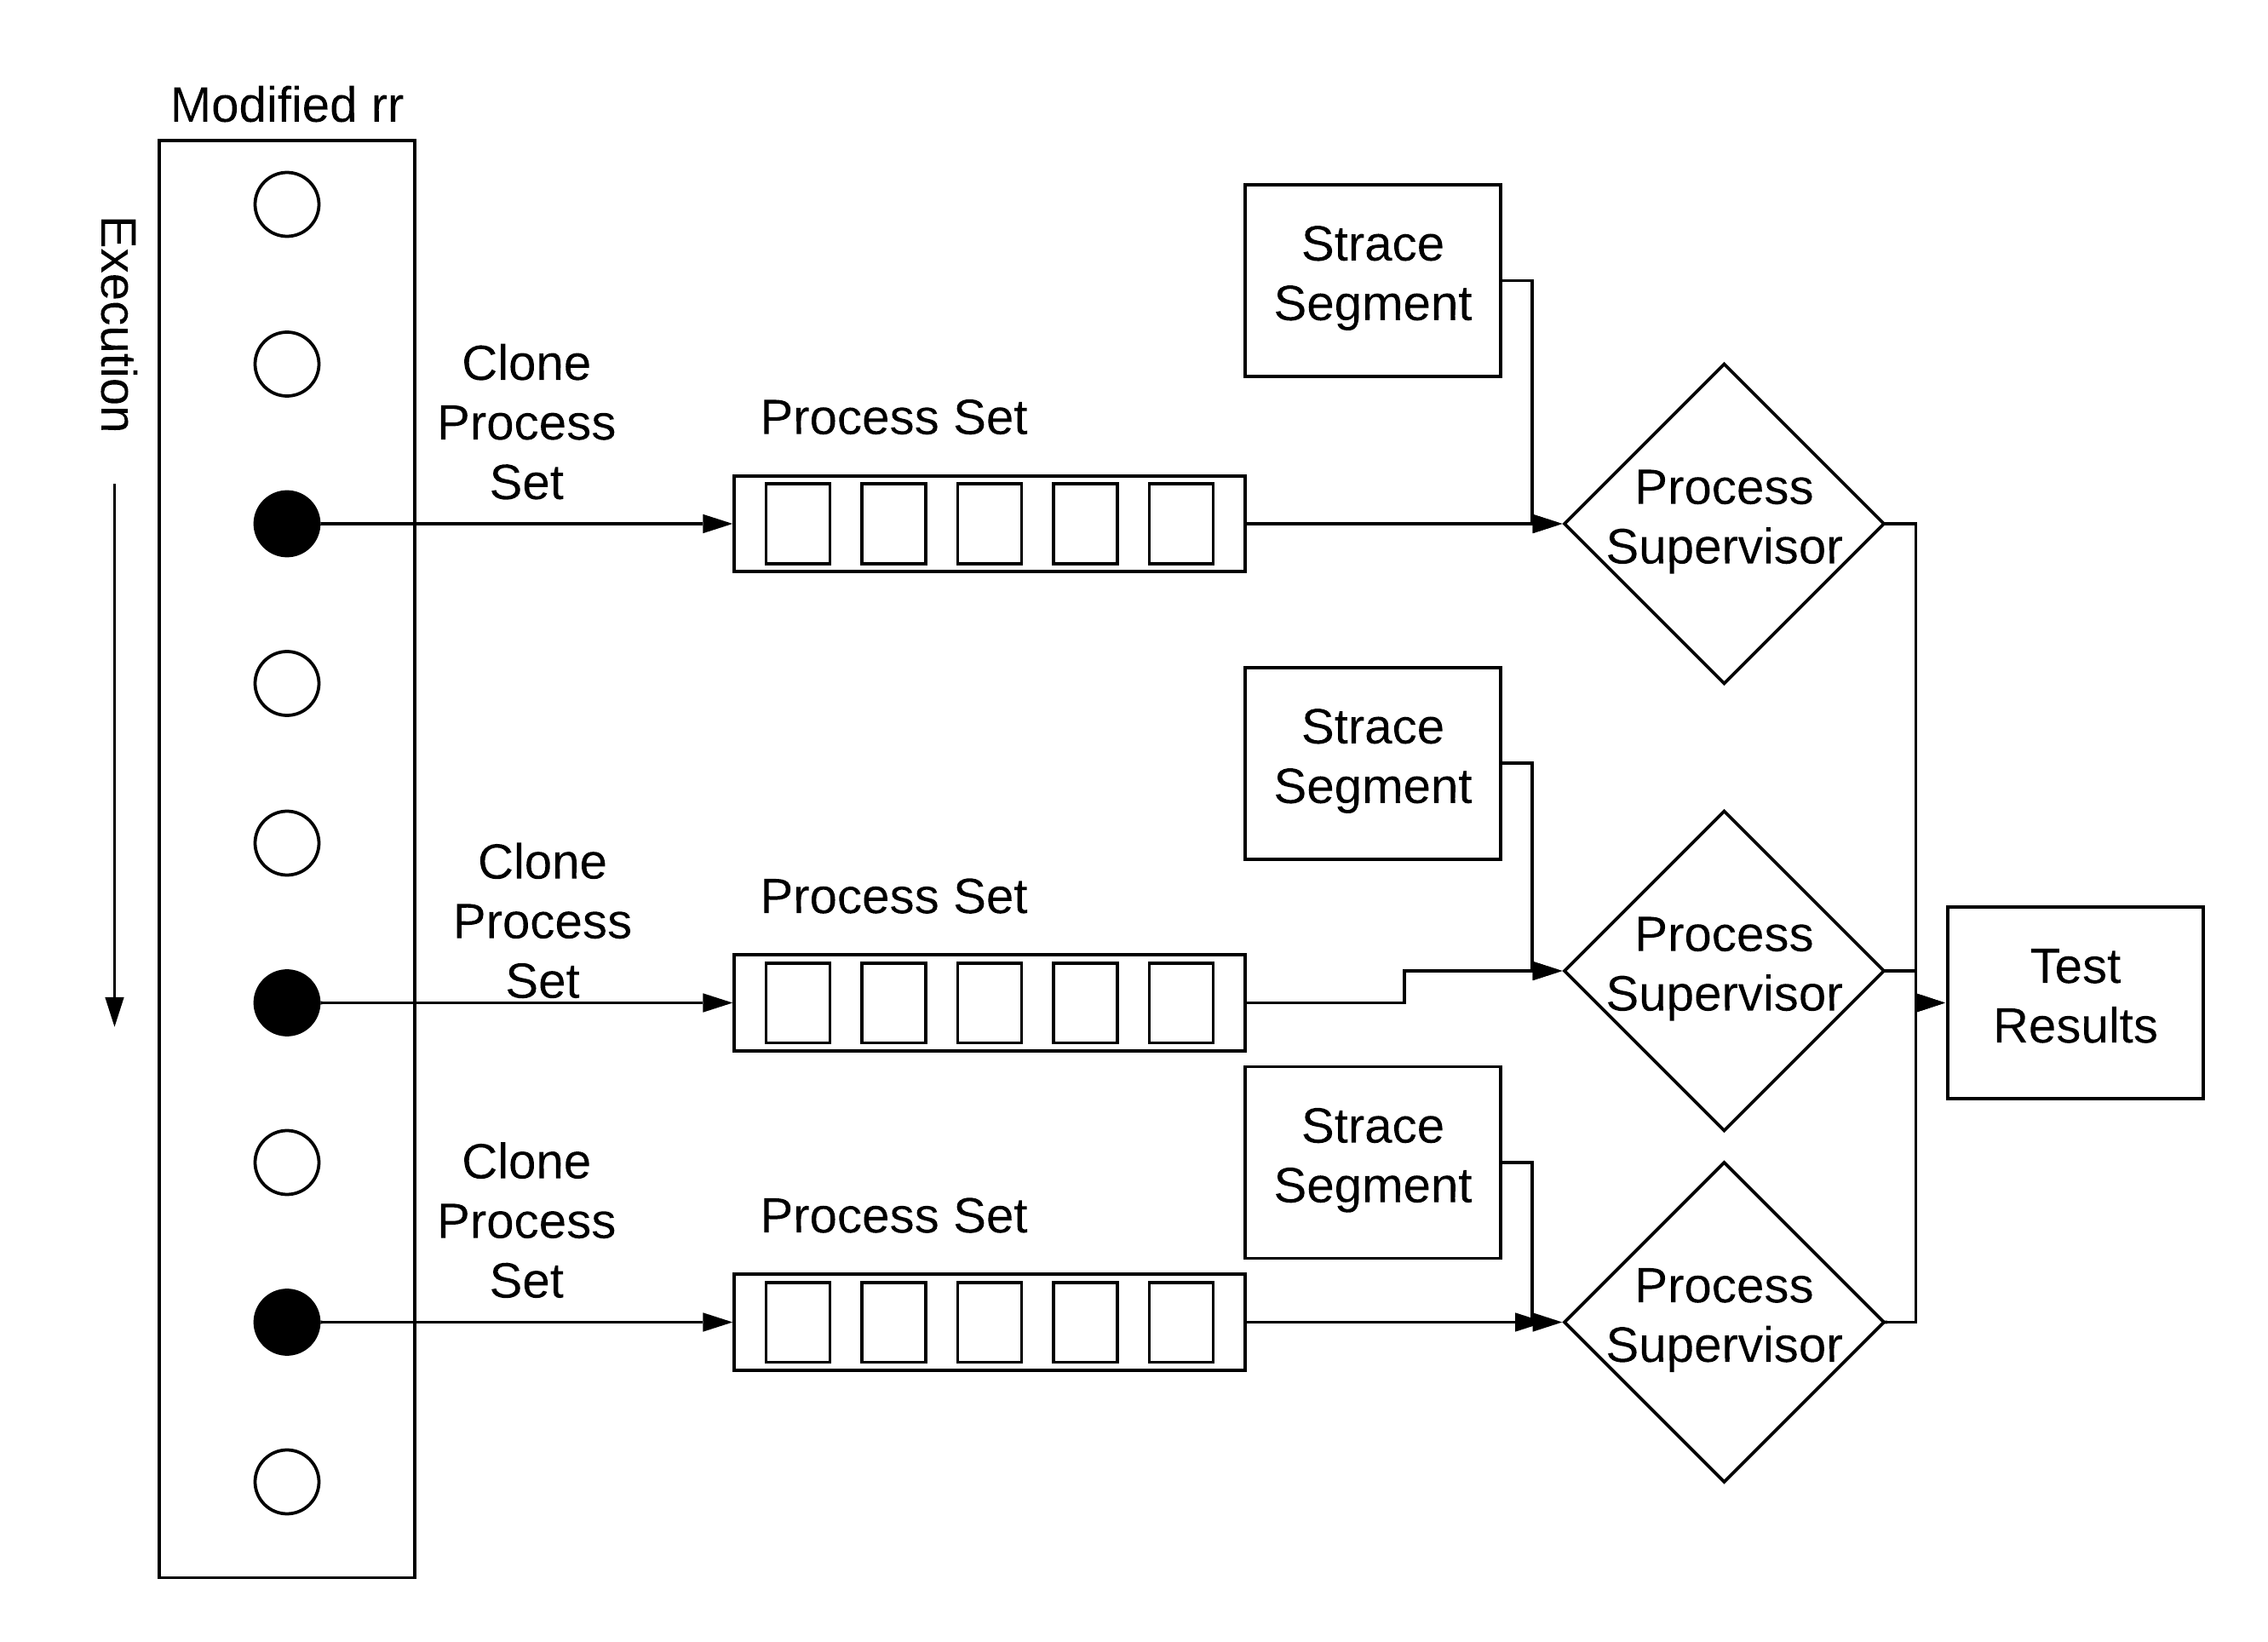
\includegraphics[scale=.65]{images/architecture}}
  \caption{Diagram illustrating CrashSimulator's Architecture.  During the
    course of a single rr execution, clone process sets are generated at
    specific rr events.  A CrashSimlator supervisor process attaches to
    these process sets and uses a strace-style system call listing to feed
    subsequent system call activity and inject unusual environmental
    conditions.}
  \label{figure:architecture}
\end{figure*}

As mentioned earlier,
the anomalous environment simulation(AES) technique
offers a reliable way to identify bugs
that could arise from interaction with a given environment.
In this section,
we will break down the steps of the technique,
and then introduce a tool called CrashSimulator,
which we built as a concrete implementation of AES.
We also describe a second technology
called Process Set Cloning
that evolved during our work on CrashSimulator.
Process Set Cloning describes an enhancement made to
the {\tt rr} debugger on which CrashSimulator was built
that allowed us to generate copies of the set of processes underlying an
application at opportune moments during replay.


\subsection{Stepping through AES}

The first step in implementing AES
is selecting an anomaly or anomalies
against which you wish to test an application.
Anomalies can be sourced
in a number of ways,
such as
examining the failures of other applications
in a target deployment environment,
or by using other tools that can identify
potentially problematic behavior in other domains~\cite{Zhuang_NSDI_2014,
rasley2015detecting}.
Public bug trackers are an ideal source
if you wish to determine
whether or not an application
is vulnerable to a widely publicized bug.
The chosen anomalies are then examined
to determine how they change an application's communications
with its environment
compared to a normal execution and why.
Once teased out,
these differences delineate
a set of modifications
that must be made to an application's communications
in order to simulate the chosen anomaly or anomalies.
Describing anomalies in this fashion
allows them to be recorded systematically and cataloged for future use.
Once captured, they can be used to repeatably test applications preventing
future deployments from falling victim to the same problem multiple
times.
As an example,
consider an anomalous environment
where access to a required file is denied because of
the environment's file security configuration.
With this anomaly,
attempts to access the file
such as calls to {\tt fread()},
or the {\tt read()} system call,
will fail with an error stating that access to the file is denied.
The ``modification'' required to simulate this anomaly
is to change the results of similar accesses
in a test execution
to return ``access denied.''
Since the effects of this anomaly have been identified, they can be saved
and used to evaluate future application's ability to handle the same
problem.

The second step in AES
is identifying
a way to monitor an application's communication
with its environment.
This can be implemented
by such means as
redirecting function calls,
observing memory access,
monitoring network activity,
or intercepting system calls.
Looking at the parameters,
return values,
and orderings
of an application's communications
can indicate
when would be an appropriate time to simulate an anomaly.
Monitoring communications
in this fashion
has the added benefit
of allowing us to find obvious situations
where an application will fail
to handle certain environmental features.
Consider an application that fails to check whether or not
a file already exists
before destructively writing to it.
The absence of this check
would be problematic in environments where the file already exists,
as it will be blindly overwritten.
The sequence of communications
the application makes when writing to the file
will make it obvious that this check has been neglected.
As such,
no simulation is required to identify the presence of a bug.

In cases such as the one described above,
the AES technique could stop at this point.
However, in most scenarios,
the last two steps ---
simulation and response analysis ---
will be required.
In the third step,
the implementer
interposes on communications
and makes the modifications necessary
to simulate the presence
of an environmental anomaly.
This could be accomplished by
influencing the results of function calls or system calls,
strategically altering memory values,
or some other method
of presenting modified communications to an application.
In the simplest case,
simulating an anomaly only requires
the modification of a single value.
In more complex cases,
large numbers of diverse communications
need to be interdicted and altered
in order to correctly simulate an anomaly.
For example,
simulating an erratic system clock
requires that all efforts
to access the clock
be modified to reflect the chosen aberration.

Lastly, the fourth AES step
is to analyze an application's response
to a simulated anomaly.
The simplest conclusion to draw
is whether or not the application
has made an effort to respond
to the anomaly,
a determination that can be made based
on the assumption
that such a response will yield
different program paths (and therefore different communications).
If the application
does not alter its behavior, it has not
correctly handled this flaw.
Alternatively,
if the application does deviate,
it is likely
an action has occurred to handle the simulated condition.
This simple yes or no approach
is often sufficient
to classify application behavior.

One limitation of the above strategy
is that it can result in false negatives
should an application change its behavior
but still not handle the anomaly correctly.
These false negatives can be addressed
by more detailed analysis
of the application's post simulation behavior.
Before testing,
a user must know
what a correct response
to an anomaly looks like.
This ``known good'' behavior can be found
by looking at standards and documentation
that describe best practices for handling an anomaly
in a given environment,
or by examining how applications that correctly
deal with the anomaly do so.
Consider the case where a {\tt close()} system call fails.
Retrying the call may not be the correct action,
depending upon the environment in question.
AES can be used to determine if an application
has handled the failure correctly
by examining post-simulation communications in detail,
and taking into account the correctness of retrying the call.

\subsection{CrashSimulator: A Concrete AES Implementation}

Evaluating AES in a real-world fashion requires a
concrete implementation of its four components.
We built this implementation into a tool we call CrashSimulator.  The
prototype was built on rr version 5.2.0 running on a 32-bit Linux kernel
distributed with Ubuntu 16.04 LTS.  The modifications to rr, which are
explained in this section, were carried out in C++ and the CrashSimulator
supervisor was implemented in ZZZZ lines of Python 2.7 code with a YYYY
line C extension that allows it to interact with processes using the Ptrace
API.
This version of CrashSimulator is available as a Docker container and,
due to some operating system configuration being necessary, is most easily
installed in this fashion.

Below, we explain the process of creating CrashSimulator, highlighting a
few central principles that guided our design decisions. The first such
decision was to operate at the system call level, rather than manipulating
calls to library functions, memory accesses, or other points where we could
influence an application's communications. Making this choice provided us a
few key advantages. First, there is already robust tooling in the Linux
kernel that allows for the interception and modification of system call
results and side effects. Additionally, Linux system call semantics are
well defined which simplifies implementation. Finally, operating at this
level allows CrashSimulator to test applications written in any language
that can execute Linux system calls.

Work then turned to gathering a corpus of anomalies to test applications
against.  These anomalies (which are further discussed
in Section~\ref{SEC:evaluation})
were collected by examining public bug trackers,
the source code of major portable applications, and the capabilities of
tools like NetCheck~\cite{Zhuang_NSDI_2014}
and CheckAPI~\cite{rasley2015detecting}.  These anomalies were converted
into sets of modified responses
that simulate the presence of an anomaly when
appropriately presented as the results of system calls.
This process required manual effort and expertise.  However,
much like
the effort involved in constructing a unit test to check for correct
behavior in a piece of code, we found that this initial outlay of
user skill and effort was paid back, as
we were able to use its products
repeatedly over time to test many different applications.

We carried out the second step of AES, communication monitoring, by
recording application executions
using a modified version of the {\tt rr}!!CITE!!
debugger.  This modification allowed
a {\tt strace}-style
system call recording to be output alongside {\tt rr's} normal recording
format, providing
a complete log of an applications system call activity.
With this information, we could
easily identify opportunities to simulate anomalies.  As was
discussed earlier, simply observing these system calls was enough to
identify bugs-of-omission in many applications
(see Section~\ref{SEC:evaluation} for a more detailed explanation).

In implementing the anomaly simulation of AES
we actually developed
a second new technique
called {\it process set cloning}.
With the modification made to rr described above,
we now can generate copies of the set of
processes underlying an application at opportune moments during replay.
The {\tt rr} debugger manages
and can copy
the full set of these
so that users can test debugging
hypotheses without damaging the original.
Our modified version
extends this capability, by liberating process sets from {\tt
rr} so that they can be exposed to simulated anomalies.
This means that we can rely on {\tt rr}
to store the information necessary to perform enough of the
replay that must take place before the application reaches the
testing point.

Process sets generated in this fashion are created in a stopped state and
remain that way until they are attached to and utilized by a CrashSimulator
supervisor.  Each process set has its own supervisor process to test
its configured environmental anomaly.  The
supervisor wakes up its designated process set
and simulates any
subsequent system calls.
During the course of this simulation, the modified responses created in
step one are supplied where appropriate,
thus exposing the processes to the
anomaly being tested.
Supervisors can complete this
process independently of one another, which lends a
high degree of speed and
parallelism to the whole CrashSimulator testing process.

The primary means by which
CrashSimulator diagnoses bugs is
by observing whether or not an application
performs a different set of system calls than what is expected based on the
recording being replayed.  A ``divergence'' from the recording indicates
the application has changed its behavior and might be handling
the anomaly in question.  Following the recording precisely, in spite of
the simulated anomaly signals the possibility of a bug.

In cases where more detailed analysis of an application's response
is required, CrashSimulator can attempt to preserve a replay execution
past the end of its recording.  This provides an opportunity for
finite automata known as ``checkers`` to examine
the system calls the application makes in order to make more detailed claims about
its response.  These checkers are discussed in more detail in our
evaluation.

\section{Implementation Details}
\label{SEC:Implementation}

\begin{figure*}[t]
  \center{}
  \fbox{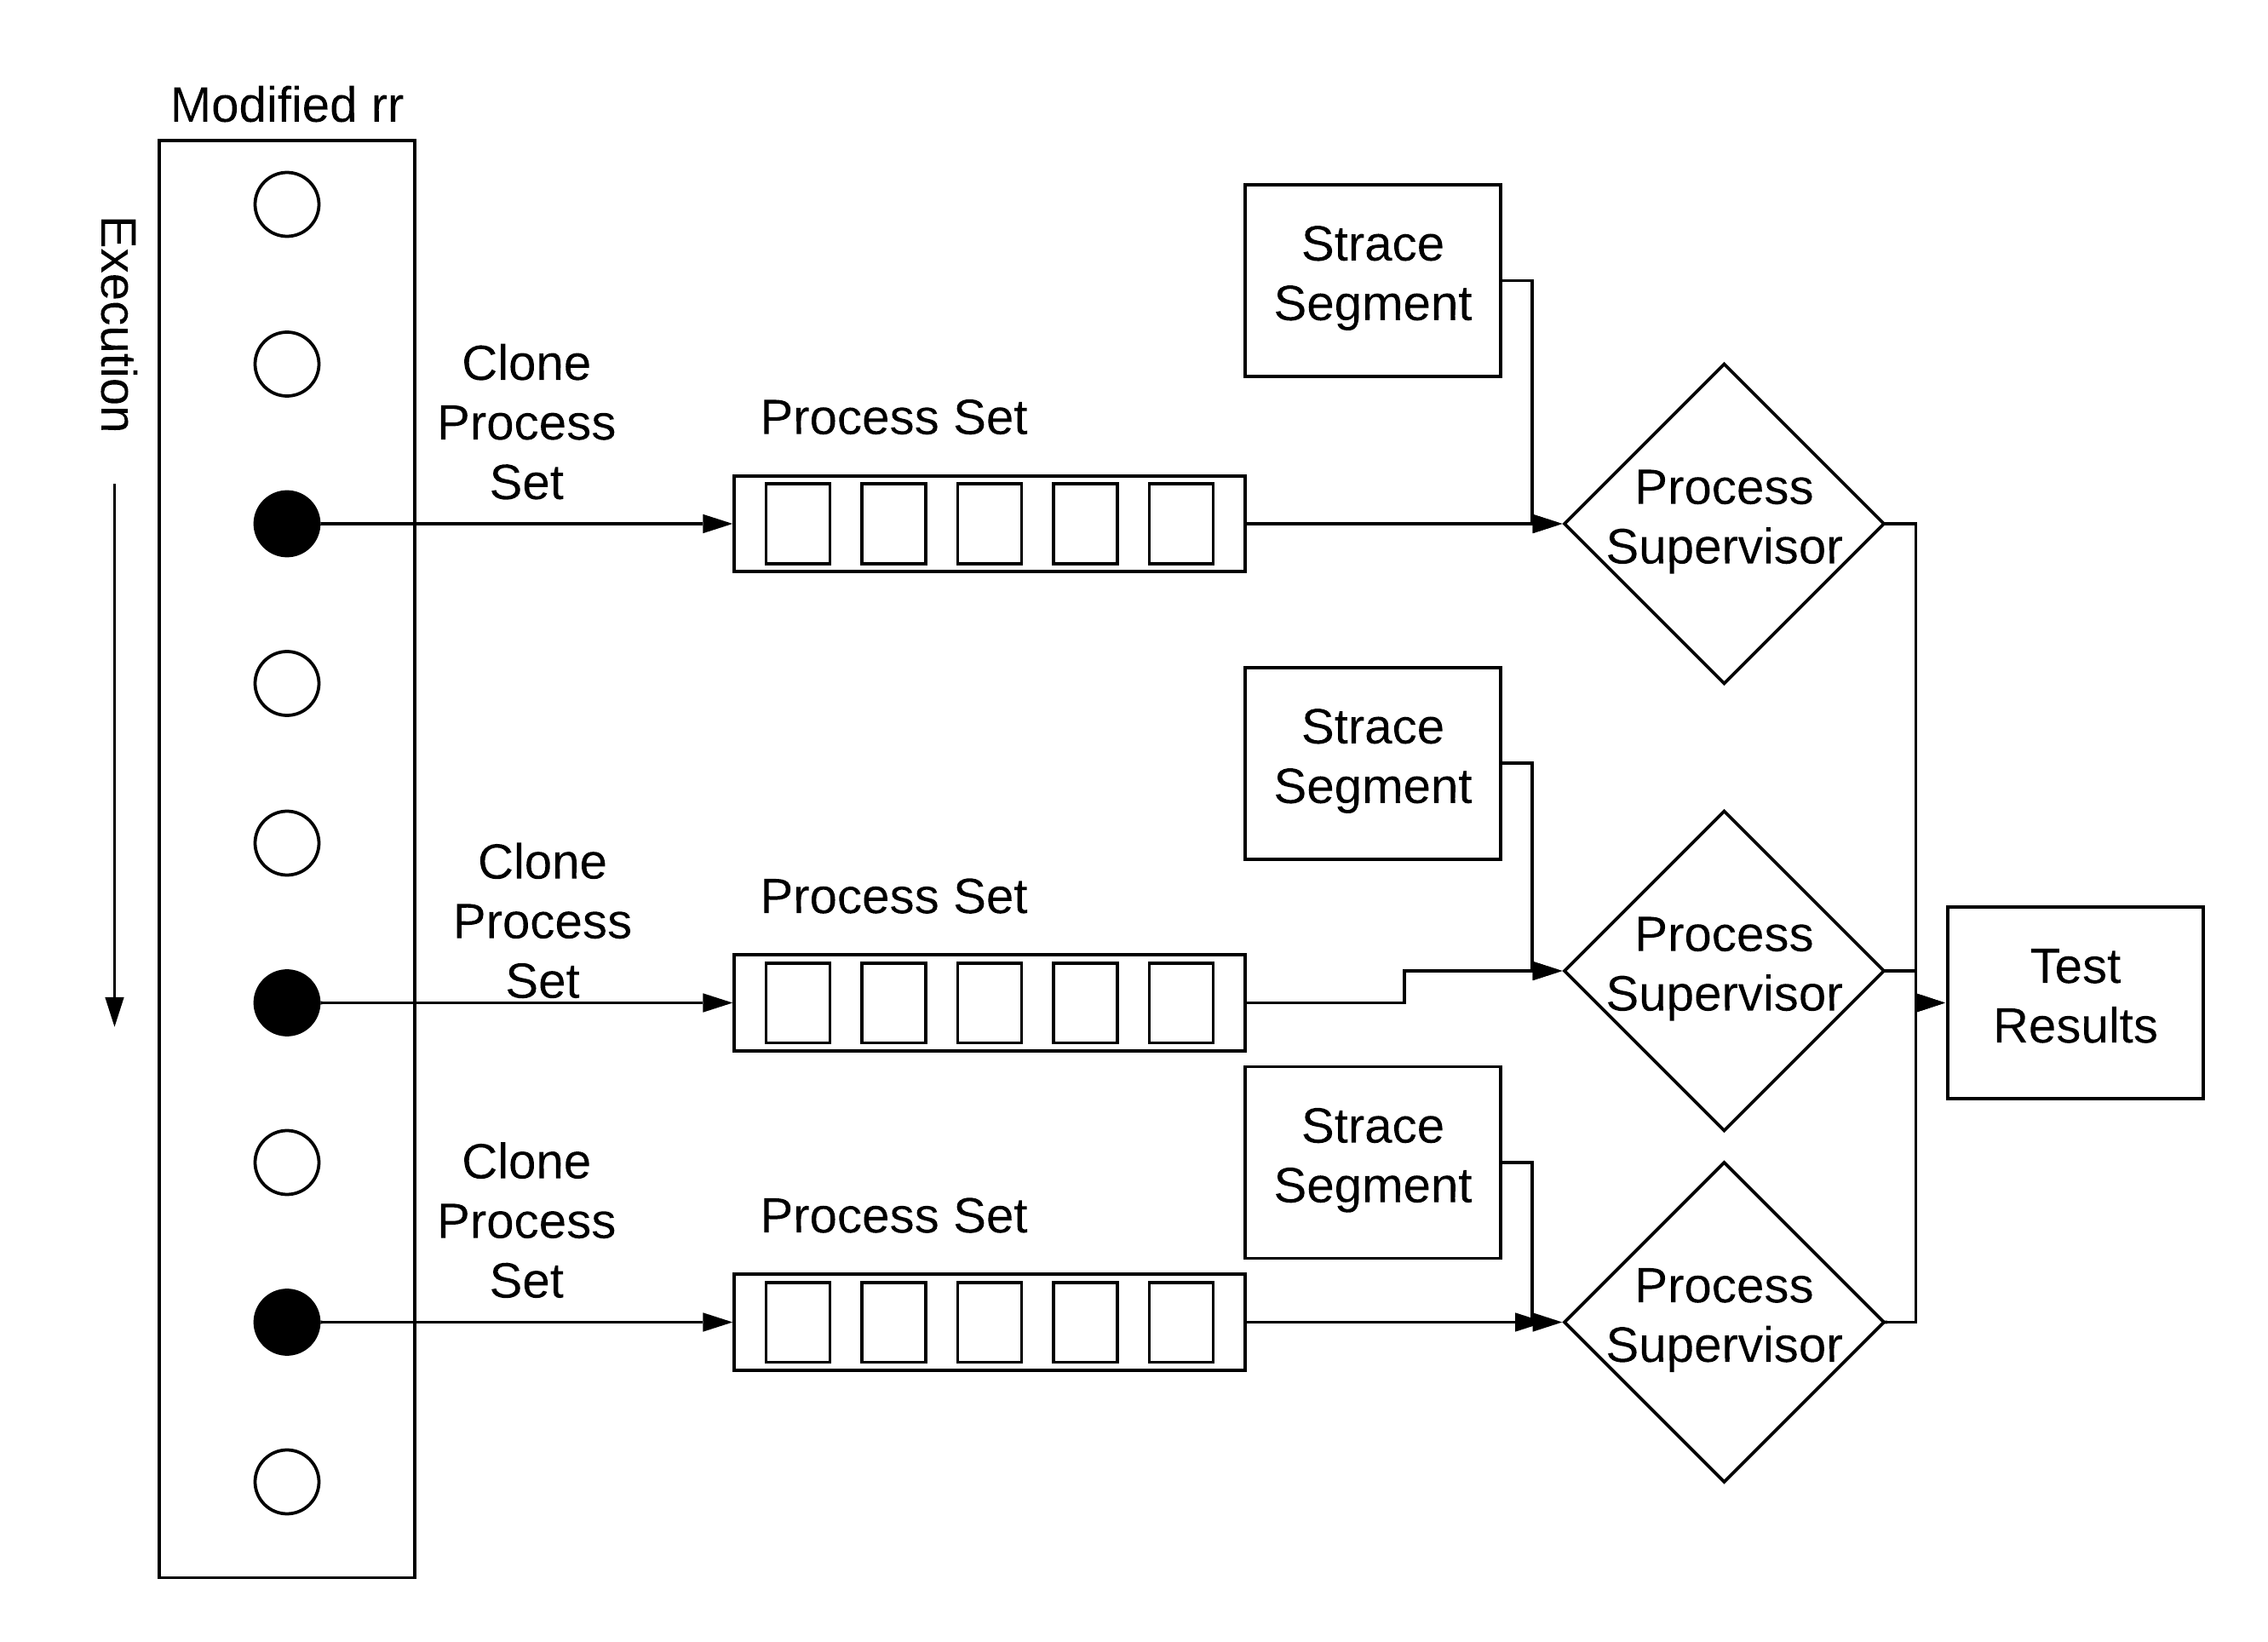
\includegraphics[scale=.65]{images/architecture}}
  \caption{Diagram illustrating CrashSimulator's Architecture.  During the
    course of a single rr execution, clone process sets are generated at
    specific rr events.  A CrashSimlator supervisor process attaches to
    these process sets and uses a strace-style system call listing to feed
    subsequent system call activity and inject unusual environmental
    conditions.}
  \label{figure:architecture}
\end{figure*}

As can be seen in Figure~\ref{figure:architecture},
our implementation of CrashSimulator uses a combination of a modified
version of {\tt rr}, a
record-and-replay debugger, and our own process supervisor
to accomplish the above.  This arrangement arose as a result of several
phases of prototyping that revealed weaknesses in more naive strategies.
Early work on an initial prototype revealed relaunching an
application and associated machinery for each test could result in
poor performance.  One of the goals of our current prototype
was so rectify this situation by eliminating as much unnecessary execution
as possible.  We achieved this by introducing a dramatic amount of
parallelism into CrashSimulator's testing process.
Central to achieving this end is the technique of
{\tt process set cloning}.  The idea behind this technique
is to generate copies
of an application's processes at specific points in execution and conduct
tests on these clones rather than the original processes.  This allows the
original processes to continue execution alleviating the need to restart
the application for each test.  This allows subsequent tests
to avoid wasting effort executing portions of the application preceding
the test.

In CrashSimulator, we implemented this technique by extending the
capabilities of the {\tt rr} record and replay debugger.  {\tt rr} manages
the full set of processes an application requires and offers the ability to
make a copy of it so that users can test debugging
hypotheses without damaging the originals.  Our modified version of {\tt
rr} extends this capability to allow process sets to be liberated from {\tt
rr} so that we can perform CrashSimulator's tests on them.
This means that we can rely on {\tt rr}
to store the information necessary to perform the bulk of
replay that must take place before the application reaches the point in
execution where testing will be performed.  When this point is reached we
take advantage of these combined capabilities
to create a
copy of the set of processes being replayed and liberate them so our
CrashSimulator process supervisor can take over replay responsibilities.

Process sets generated by {\tt rr} are created in a stopped state and
remain until they are attached to and utilized by a CrashSimulator
supervisor.  Each process set has its own supervisor process to inject
its configured environmental anomaly.  The
supervisor wakes up the process set it is managing and simulates any
subsequent system calls it makes.  The data necessary for this
simulation is
supplied as a system call listing formatted after the style of {\tt strace}
output, that describes the results and side effects for each system
call. The output is engineered in such a way to contain the
elements required to reflect the
desired environmental anomaly.  Supervisors can complete this
process independently of one another, which lends a
high degree of speed and
parallelism to the whole CrashSimulator testing process.


\subsection{Mutators and Test Portability}

A second problem discovered in earlier prototypes was the difficulty of
sharing tests between developers.  Differing system hardware and software
setups meant that recordings taken a two different machines could vary
enough that anomaly injection opportunities would occur at unpredictable
spots in a recording.  A universal method for detecting these opportunities
was needed in order to address these situations.  The successful strategy
we landed upon was encoding anomaly injection opportunities as finite
automata that consume the ordering and attributes of system calls in a
recording.  These automata allow a mutator script to correctly identify
these opportunities regardless of where they occur as a result of variances
in test machines.  At the same time, this capability is what allows tests
constructed for CrashSimulator to be used across applications.

\subsection{Improving the CrashSimulator's Capabilities}
\label{sec-improving-tool}

CrashSimulator's users are able to improve its capabilities through
the addition of new anomalies.  This process involves identifying a new
anomaly, transforming it into a set of system call results and side
effects, and implementing a mutator script that CrashSimulator can use in
testing applications.

\subsubsection{Converting Anomalies to System Call Sequences}

Once a new anomaly has been identified, it is distilled into a
representative set of system call results and side effects.
This process involves examining the
system calls made by an application running in the anomalous environment
and selecting a set of modifications that, when applied to a recording,
simulate the presence environmental condition in question.
This process requires manual effort and expertise.  However,
much like
the effort involved in constructing a unit test to check for correct
behavior in a piece of code, this initial outlay of
user skill and effort will be paid back, as it is
used repeatedly over time to test many different applications.

As a more concrete example of the above, consider an anomaly
involving unusual file types we will later address in our evaluation of
CrashSimulator.
This anomaly appears when a call to {\tt stat()} or a similar system
call returns a structure with a {\tt st\_mode}
member containing an unexpected
value. Consider the line of {\tt strace} output representing a call to {\tt
  fstat()}:
\begin{quote}
  {\tt 8936  fstat64(3, \{st\_dev=makedev(0, 40), st\_ino=54993216, st\_mode=S\_IFREG ...\}) = 0}
\end{quote}
The third member of the returned structure indicates that the file is a
regular file by showing that {\tt st\_mode} flag is set in the {\tt st\_mode}
member.  CrashSimulator can mutate this  line to the following:

\begin{quote}
  {\tt 8936  fstat64(3, \{st\_dev=makedev(0, 40), st\_ino=54993216, st\_mode=S\_IFCHR ...\}) = 0}
\end{quote}

The trace containing this modified line can then be replayed in order to
test how the application responds when a file that is expected to be
regular is actually a character device. In our evaluation, we further
explore the behavior of applications as they encounter other possible valid
values of {\tt st\_mode} in the course of testing.

\section{Evaluation}
\label{SEC:evaluation}

CrashSimulator was designed
as a way to reduce the considerable effort
required of developers
in implementing and maintaining applications.
Therefore,
we needed to prove its effectiveness in ``the wild.''
To this end,
we planned two rounds of
evaluation for CrashSimulator.
We started by exposing
a series of real-world applications
to a library of collected anomalies in a laboratory environment.
These tests,
conducted by the research team,
were followed by a user study
in which undergraduate and graduate computer science students
got a chance to use CrashSimulator
to identify new environmental bugs
in tests on applications of their choosing.
We used the results from both these efforts
to answer the following questions:

\begin{enumerate}

\item{Is CrashSimulator able to identify a wide variety of environmental
    bugs?
(Subsection~\ref{sec-env-bugs})}

\item{What Sorts of Errors Does CrashSimulator Make?
    (Subsection~\ref{sec-sorts-errors})}

\item{Can CrashSimulator
      execute tests efficiently? (Subsection~\ref{sec-perf})}

\end{enumerate}

\subsection{Is CrashSimulator able to identify a wide variety of
environmental bugs?}
\label{sec-env-bugs}

The most crucial question to ask about CrashSimulator
is how readily it can
identify bugs
caused by a wide variety of environmental differences.
We have already established
that these bugs can arise from
unusual filesystem and network situations,
so we configured the tool to look
for bugs that could be triggered by these features.
These bugs rely on common system calls,
and thus had the potential to
appear in many programs.
As we wanted to test
the most commonly used applications,
our selections were made
from among those deemed ``popular''
by Debian's Popularity Contest~\cite{DebPopCon},
or those used
by many Linux distributions,
such as ones provided
by the GNU Coreutils project.

\subsubsection{The simplest case - A Filesystem Bug Found With the Null Mutator}

In our first test we decided to evaluate the tool in its simplest possible
configuration -- employing the null mutator.
This mutator takes no action and simulates no anomalous conditions.
It simply allows checkers
a chance to evaluate an application's behavior
as it carries out a potentially-buggy operation unhindered.
To test CrashSimulator's ability to find bugs
in this fashion, we decided to look at how applications
move files about on the filesystem.
In many cases this operation can be handled
atomically by the operating system
through the {\tt rename()} system call.
However,
in situations where the source file and destination file
are on different storage devices,
the application must
manually perform all of the required steps.
This is a process
that even well-tested applications
frequently get wrong~\cite{PHPRenameBug,PythonShutilBug,NodejsCopyBug}.

{\bf Method.}  For this portion of our evaluation
CrashSimulator was configured
to test each of the applications listed in Table~\ref{table:crossdevice}
using the Null Mutator and a set of checkers constructed find applications
that fail to correctly move a file from one disk to another.
Catching this particular class of bugs requires
checkers that encode the correct steps involved in moving a file from one
storage device to another.
After examining several libraries and applications,
we found that
{\tt mv} seemed to handle cases that other tools failed to consider.
Therefore, we
used its behavior as a template to create a set of checkers
that evaluate whether or not
the application correctly performs the following
types of checks and operations:

\paragraph{Source Replaced.}

An application should make an effort
to ensure that the file being copied
is not replaced between the time it is initially examined
and the time it is opened for copying.
Otherwise,
it could have been replaced by a file of a different type,
such as a character device.
To test whether applications are robust
to anomalies involving source file replacement,
we developed a checker that monitors whether a series of safety checks
are performed.
If these checks are not performed it
means the application will proceed with its operations,
leaving open the possibility of file corruption~\cite{PythonShutilBug}.

\paragraph{Preserve Xattrs}

Extended file attributes
are used by modern operating systems
to store descriptive information
that the strictly defined and limited structure
of normal filesystem fields cannot hold.
For example,
an operating system can use extended file attributes
to record whether or not a file was downloaded from the Internet.
This is important security information
that is used to warn users
if they are about to open a potentially unsafe file.
Apple's Gatekeeper relies on extended file attributes
to prevent the execution of applications downloaded from
untrusted developers without explicit user action~\cite{AppleCodeSigning}.
When copying a file,
an application should retrieve extended file attributes from the source
file and, later, apply them to the destination file.
In this case, CrashSimulator used a checker
that watches for the application to make system calls
that read the extended file attributes from the source file (i.e. {\tt
  getxattr()}, {\tt lgetxattr()}, or {\tt fgetxattr()}) followed by system calls
that re-apply the attributes to the destination file (i.e. {\tt setxattr()},
{\tt lsetxattr()}, or {\tt fsetxattr()}).

\paragraph{Preserve Timestamps}

Incorrect timestamps can impede applications like
in {\tt make}, archival programs, and similar
software~\cite{NautilusTimestamps, SudoTimestamp}.
As a result, it is important to ensure
that time related metadata --
such as creation, modification, and access times
are preserved when copying a file.
To evaluate failures on this front,
we used a checker that determines
whether the application applies
the appropriate timestamps to the destination file
by monitoring for system calls from the {\tt stat()}
and {\tt utime()} families used to retrieve and apply timestamps.

\paragraph{Copying Devices}

It is also important to check if a move
would attempt to copy a special
device file, such as a named pipe, across disks.
Files of this variety must be moved
by creating a new device of the same type at the destination,
instead of exhaustively reading and writing its contents.
In our experience, applications that fail to perform this check
can end up completely filling a disks, exhausting available memory,
or blocking forever, which can cause the system to become unresponsive.


 \begin{table}[t]
    \scriptsize{}
    \begin{tabular}{l p{1cm} p{1cm} p{1.2cm} p{1cm}}
    \toprule{}
        Application     & Source Replaced & Preserve Xattrs & Preserve Timestamps & Copying Devices\\
\hline
        {\tt mv}              & Correct             & Correct         & Correct             & Correct\\
        {\tt mmv}             & Correct             & {\bf Sec. Flaw} & {\bf Time Loss} & Correct\\
        {\tt install}         & Correct             & {\bf Sec. Flaw} & {\bf Time Loss} & {\bf Fill Disk} \\
        {\tt perl File::Copy} & Correct             & {\bf Sec. Flaw} & {\bf Time Loss} & {\bf Fill Disk} \\
        {\tt shutils}         & {\bf Corrupt}	& {\bf Sec. Flaw} 	& Correct             & Correct\\
        {\tt rust}             & Correct             & {\bf Sec. Flaw} & {\bf Time Loss} & {\bf Fill Disk} \\
        {\tt boost::copyfile} & {\bf Corrupt}	      & {\bf Sec. Flaw} & {\bf Time Loss} & {\bf Fill Disk} \\
    \bottomrule{}
    \end{tabular}
    \caption{Applications and libraries analyzed to determine whether or not
      they are able to correctly move a file from one device to another.
Incorrect entries are either missing the needed check or were ineffective.}
    \label{table:crossdevice}
\end{table}

{\bf Findings.}
As can be seen from the results in Table~\ref{table:crossdevice}, each of the
applications tested fails to perform one or more of the steps required to
successfully complete a cross-device move.  This is an unfortunate situation
because a failure to perform any one of these steps can result in negative
outcomes for the system as a whole.
Our results indicate that CrashSimulator is able to identify whether complex
operations are performed correctly in anomalous situations in
an array of popular programs.
This includes the standard libraries for the programming languages Python,
Perl, and Rust, along with other widely used software.  This is true even
when many libraries have correct behavior in some cases, but not others.


\subsubsection{A More Complex Case - The Unexpected File Types Mutator}
\label{sec-file-type-bugs}

Employing a mutator
with more complexity than the null mutator
allows CrashSimulator to inject anomalies into an execution
of an application.
This introduces problematic scenarios
so that the way an application responds
can be evaluated.
To test
the tool's capabilities
at this point,
we needed an anomaly
that would arise during a common situation,
such as when a Linux application retrieves
and processes data from a file.
Linux supports
several special file types,
including
directories,
symbolic links,
character devices,
block devices,
sockets, and
First-In-First-Out (FIFO) pipes.
These special files
use the same system calls
as regular files
(such as {\tt read()} and {\tt write()}),
but they behave in very different ways.
For example,
{\tt /dev/urandom} is a character device
that produces an infinite amount
of pseudo-random data
when read.
If an application that reads the full
contents of a file before processing is provided {\tt /dev/urandom}, it
will fill memory or disk space and could
crash the system~\cite{YumAptEndless}.
Correct execution in these situations
requires applications
to examine the files so they do not
interact inappropriately with a given file type.

{\bf Method.} In order to confirm the accuracy of CrashSimulator's assessments we
exposed a subset of the Coreutils applications tested to
a simulation of the unusual file
types to get an idea of how they would respond.
Identifying these bugs involves changing an application's
execution to induce its response to an unexpected file type.  For
example, the {\tt sed} application, which modifies the contents of a text
file according to a provided command string, could be provided a symbolic
link, a directory, or a character device instead.  CrashSimulator
accomplishes this by identifying the calls to {\tt stat()}, {\tt fstat()},
or {\tt lstat()} that an application makes to examine the file, and then
changing their results to simulate
one of the special file types.  If the application responds to
this injected information then there is the possibility that the special
file will be handled correctly.  On the other hand, if there is no
alteration in the behavior of the application,  then the condition is not
being handled correctly.

For each application,
CrashSimulator was configured to simulate all of the non-standard file
types and
Table~\ref{table:unexpectedtypes} shows the values that CrashSimulator
inserted into the results of the {\tt stat()}-like calls made by the
application.
A result of ``Expected Type (ET)'' indicates
that this is the file type the application was provided
when the application was initially recorded -- that is,
a file of the type the application was expecting.
A result of ``\tickmark'' indicates that the application
identified it was being provided with an unexpected file type and its
execution diverged,
indicating that it was potentially handling the
unexpected file type correctly.
A result of ``\xmark'' indicates that the
application failed to recognize the presence of the unusual file type
because execution never diverged from the trace being replayed.
We manually examined a subset of the listed application behaviors simulated by
CrashSimulator and verified they were consistent with the actual behavior
on the given file type.

{\bf Findings.}

The frequency of failed executions in our results,
which are shown in Table 2,
indicates that many
applications make the assumption that they will only be used to process
regular files.  When this assumption does not hold, execution results
can be hard to predict.
In many cases a denial of
service condition occurs in the form of the application ``hanging,'' as it
attempts to incorrectly process the file.
This may happen harmlessly, such
as if an application blocks forever waiting for a {\tt read()}
call to retrieve non-existent data from an empty FIFO,
or harmfully,
as when an application attempts to read in and process an
``infinitely large'' file,
that will eventually fill all
available memory or disk space~\cite{Cappos_CCS_08}.


\begin{table*}[t]
    \scriptsize{}
    \begin{tabular}{l  l  |  l  l  l  l  l  l  l}
    \toprule{}
        Application       & Condition Tested           & Regular File & Directory & Character Device & Block Device & Named Pipe & Symbolic Link & Socket File (IFSOCK)\\
                          &                            &  (IFREG)     & (IFDIR)   & (IFCHR)          & (IFBLK)      & (IFIFO)    & (IFLNK)       & (IFSOCK)\\
\hline
        {\tt Aspell}      & Dictionary File            & ET        & \xmark     & \tickmark  & \xmark    & \xmark        & \xmark       & \xmark\\
        {\tt Aspell}      & File being checked         & ET        & \xmark     & \tickmark  & \xmark    & \xmark        & \xmark       & \xmark\\
        {\tt gnu-gpg}     & secring.gpg                & ET        & \xmark     & \xmark     & \xmark    & \xmark        & \xmark       & \xmark\\
        {\tt vim}         & File being opened          & ET        & \tickmark  & \tickmark  & \tickmark & \tickmark     & \tickmark    & \xmark\\
        {\tt nano}        & File being opened          & ET        & \tickmark  & \tickmark  & \tickmark & \xmark        & \xmark       & \xmark\\
        {\tt sed}         & File being edited          & ET        & \xmark     & \tickmark  & \xmark    & \xmark        & \xmark       & \xmark\\
        {\tt df}          & /proc                      & \xmark    & ET         & \xmark     & \xmark    & \xmark        & \xmark       & \xmark\\
        {\tt wc}          & File being checked         & ET        & \tickmark  & \tickmark  & \tickmark & \tickmark     & \tickmark    & \tickmark\\
        {\tt du}          & Directory being checked    & \tickmark & ET         & \tickmark  & \tickmark & \tickmark     & \tickmark    & \tickmark\\
        {\tt install}     & File being installed       & ET        & \tickmark  & \xmark     & \xmark    & \xmark        & \tickmark    & \xmark\\
        {\tt fmt}         & File being formatted       & ET        & \xmark     & \tickmark  & \xmark    & \xmark        & \xmark       & \xmark\\
        {\tt od}          & File being dumped          & ET        & \tickmark  & \tickmark  & \xmark    & \xmark        & \xmark       & \xmark\\
        {\tt ptx}         & File being read            & ET        & \tickmark  & \tickmark  & \tickmark & \tickmark     & \tickmark    & \tickmark\\
        {\tt comm}        & Second file being compared & ET        & \tickmark  & \tickmark  & \xmark    & \xmark        & \xmark       & \xmark\\
        {\tt pr}          & File being read            & ET        & \tickmark  & \xmark     & \xmark    & \xmark        & \xmark       & \xmark\\
\hline
        \multicolumn{9}{l}{\scriptsize{\tickmark  $=$ CrashSimulator
        predicts application will recognize anomaly}}\\
        \multicolumn{9}{l}{\scriptsize{\xmark  $=$ CrashSimulator predicts
        application will fail to recognize anomaly}}\\
        \multicolumn{9}{l}{\scriptsize{ET (Expected Type)  $=$ File type expected by the
        application}}\\
    \bottomrule{}
    \end{tabular}
    \caption{Applications tested for their handling of unexpected file types.  A
    result of ``\tickmark'' indicates that the application identified the
    presence of an unusual file and responded in some fashion.  A result of
    ``\xmark'' indicates that the application failed to recognize the presence of
    an unusual file and attempted to process it.}
    \label{table:unexpectedtypes}
\end{table*}


\begin{table*}[t]
    \scriptsize{}
    \begin{tabular}{l  l  l  l  l  l  l  l  l}
    \toprule{}
        Application         & Directory                 & Character Device & Block Device  & Named Pipe \\
        Application         & (IFDIR)                   & (IFCHR) & (IFBLK) & (FIFO) \\
\hline
        {\tt wc}            & Error: Is a Directory     & hangs       & slowly process file  & Hangs\\
        {\tt install}       & Error: Omitting Directory & Fills disk  & slowly copies file   & Hangs\\
        {\tt fmt}           & No output                 & hangs       & garbage output       & Hangs\\
        {\tt od}            & Error: read error         & hangs       & No output            & Hangs\\
        {\tt ptx}           & Error: Is a Directory     & fills disk  & garbage output       & Hangs\\
        {\tt comm}          & Error: Is a Directory     & hangs       & garbage output       & Hangs\\
        {\tt pr}            & Error: Is a Directory     & hangs       & garbage output       & Hangs\\
\hline
    \bottomrule{}
    \end{tabular}
    \caption{Responses of a sample of coreutils applications when exposed to
      anomalous conditions.  The character device used was the infinite-length {\tt
        /dev/urandom}.}
    \label{table:applicationresponses}
\end{table*}


Table~\ref{table:applicationresponses} contains the results of this test.
CrashSimulator's evaluation of an application can map to real world bug behavior
in a few different combinations
One
possibility is that CrashSimulator asserts that the application will fail
and in practice, it does.  This is the case when we evaluated
the response of  {\tt install} being provided a character device
rather than a regular file. CrashSimulator predicted failure and the
application ended up filling the disk of the machine on which it was run.  The
opposite can also occur.  That is, CrashSimulator reports that the
application detected the anomalous condition and the application manages to
do so in practice,  as when we evaluated {\tt wc}'s successful response to
being run on a directory.

\subsubsection{Beyond Filesystem Bugs - Poorly Configured Network Timeouts}
\label{sec-timeout-bugs}

CrashSimulator is not limited
to identifying filesystem-based anomalies.
The third anomaly we examined
involves an application's behavior
when it attempts to communicate
over a network with extremely long
(on the order of minutes) response times.
At a low level,
applications retrieve data from a network socket
by waiting for data to be available and then reading it.
However,
this approach needs to be able to handle
a situation where communication
takes too long and should time out.

{\bf Method.} CrashSimulator can detect
whether an application is vulnerable to this attack
by employing the null mutator and a network timeout checker
in order to determine if it makes any effort
to configure its network communications with a timeout value.
This is done
by examining the presence or absence of {\tt setsockopt()}, {\tt poll()}
and {\tt select()} calls as well as the timeout values that may
have been passed to them. Applications that do not set the timeout are
subject to the operating system-defined protocol timeout value (19 minutes
on Linux).
CrashSimulator is able to take this analysis a step further by employing a
Long Network Response Time mutator
that manipulates
the results of all time-returning calls,
simulating an execution where close
to the maximum timeout value occurs,
without actually spending any time
waiting.

An application's failure
to time out responsibly
is not just an inconvenience --
it can be taken advantage of by attackers
to consume resources and potentially cause a denial of service situation.
This failure was exploited by the slowloris~\cite{Slowloris} tool
to enhance the ability
of a small number of computers to prevent access
to vulnerable web servers
by opening and maintaining connections to the servers
for extremely long periods of time.
As these servers could only handle a set number of connections
due to resource constraints,
legitimate traffic was easily crowded out by the attackers.
Additionally, similar attacks can be used to
indefinitely delay security updates to
clients, leaving them vulnerable to compromise~\cite{Cappos_TR_08}.
We used CrashSimulator to determine which applications and
libraries from a selection based on Debian's ratings~\cite{DebPopCon}
could be vulnerable to this sort of attack.

\begin{table}[t]
  \scriptsize{}
  \begin{tabular}{l | l}
    \toprule{}
    {\bf Application}              & {\bf Analysis Result}\\
    {\tt wget}                     & Overly long timeout supplied to {\tt select()} \\
    {\tt ftp}                      & No {\tt poll()} or {\tt select()}, no timeout set \\
    {\tt telnet}                   & {\tt select()} specifies no timeout \\
    {\tt urllib http}              & No {\tt poll()} or {\tt select()}, no timeout set \\
    {\tt urllib ftp}               & No {\tt poll()} or {\tt select()}, no timeout set \\
    {\tt ftplib}                   & No {\tt poll()} or {\tt select()}, no timeout set \\
    {\tt httplib}                  & No {\tt poll()} or {\tt select()}, no timeout set \\
    {\tt requests}                 & No {\tt poll()} or {\tt select()}, no timeout set \\
    {\tt urllib3}                  & No {\tt poll()} or {\tt select()}, no timeout set \\
    {\tt python-websocket-client}  & No {\tt poll()} or {\tt select()}, no timeout set \\
    \bottomrule{}
  \end{tabular}
  \caption{Applications tested for their handling of extremely slow response
    times from the host with which they are communicating }
  \label{table:slowloris}
\end{table}


{\bf Findings.} As Table~\ref{table:slowloris} shows, all of these
applications were vulnerable to this sort of anomaly,
and in some cases,
the timeouts took hours to resolve.
What's more, in the vast majority of
cases, the problem occurs because the application makes no effort to
specify a timeout value.  This means an attacker can transmit one byte of
data per timeout period (per Linux's value of 19 minutes for TCP sockets),
allowing them to keep the application alive instead of quitting.

\subsubsection{Bugs Found By Participants}

Another topic of relevance
in evaluating CrashSimulator
is how well developers are able to use the tool
to find bugs.
To investigate this angle
we conducted a user study
with 12 undergraduate and graduate students.
These students had varying levels
of operating systems experience
and minimal training with the tool.
Still, study participants found a total of 11 bugs using CrashSimulator.
Of these bugs, nine were found using the ``Unusual Filetype'' mutator.
Five of these bugs have since been reported to the appropriate maintainers,
and three of these reports included patches built by the reporting student
that correct the bug.

These results are important
because they confirm
users other than the original development team
for CrashSimlator
can use it to find new bugs in real world applications.
Participants commented that narrowing the source of a bug
down to a particular sequence of system calls
was helpful in identifying the area of
code responsible for the bug -- a feature
that decreased the time required to produce a fix.
Though observation of study participants
showed that familiarity with operating systems concepts
made it easier to work with CrashSimulator,
those without this background were still able to identify bugs using the
built in anomalies.


On a less positive note,
the study did reveal
some shortcomings
of the tool.
First,
it revealed that the tool
does not have a clear mechanism
for determining
what application behaviors constitute a bug.
For example,
it may be the intention of an application's developer
to have the application run continuously
until killed by an outside command
when processing an ``infinitely long'' file,
and therefore that behavior should not be classified as a bug.
Second,
it demonstrated that
simply reporting an application did or did not change its behavior
in the presence of an anomaly is insufficient
if CrashSimulator's user is unfamiliar
with what each result indicates in terms of the presence of a bug.
Both of these issues are being corrected
by improving what the tool outputs.
By more clearly describing
the nature of a given result,
users can have a better idea
if,
and why,
they should be concerned.


\subsection{What Sorts of Errors does CrashSimulator Make?}
\label{sec-sorts-errors}

\textbf{False Positives.}
Like most other testing tools, CrashSimulator occasionally makes
false positive reports.
Because these errors waste developer time and effort,
being able to adjust CrashSimulator to eliminate them when they are
encountered is a key concern.
The primary source of false positives in CrashSimulator is an application
using a different sequence of system calls to implement a given operation
than was expected by mutator.
CrashSimulator's approach allows these
situations to be easily corrected, once identified.
This is similar to the circumstance where an
application's test suite is missing a test, necessitating action by the
developer to construct it.

For example, consider GNOME's {\tt glib} file handling functions.  When an
application makes use of these facilities to move a file across storage
devices the library itself correctly performs a
file move operation.  When we used CrashSimulator with
checkers that expected a calls to {\tt read()} and {\tt write()}
for a cross-device move, we got reports stating that the
application {\em did not} perform the system calls necessary to inject
an anomaly.  By manually
examining a system call trace, we found that, while {\tt glib} correctly
performs the requested move operation,
it does so using alternative system call
sequences.  Rather than using a sequence of {\tt read()} and {\tt write()}
calls, as our checker expected, {\tt glib} creates a pipe and uses the {\tt
splice()} system call to copy the contents out of the source file, through
the pipe and into the destination file.

Fortunately, as soon as issues like this are discovered,
CrashSimulator's checkers can be modified to include the alternative
approach.  This is viable because there
are a finite number of system calls, and a given operation can be mapped to
a manageable subset.  Given the above example around moving
files, consider the mapping from high level ``operation'' to the set of
system calls that can implement it in Table~\ref{table:stepsandcalls}.
Each of the steps in the operation map to a small number of system calls
and,
in
situations where two system call sequences can correctly implement the same
operation, CrashSimulator simply runs two checkers in parallel resulting in a
test executing for the one whose prerequisites are met.

\begin{table}[t]
    \scriptsize{}
    \begin{tabular}{l | l }
    \toprule{}
      {\bf Operation}                                               & {\bf Potential System calls}\\
      Examine source file                                     & stat64(), lstat64(), fstat64()\\
      Examine destination file                                & stat64(), lstat64(), fstat64()\\
      Open source file                                        & open()\\
      Read contents of source file                            & read(), splice() with a pipe\\
      List source file's & \\ ~~~~~extended file attributes             & listxattr(), llistxattr(), flistxattr()\\
      %Read contents of source file's extended file attributes & getxattr(), lgetxattr(), fgetxattr()\\
      Read contents of source file's                    & \\
      ~~~~~~~extended file attributes & getxattr(), lgetxattr(), fgetxattr() \\
      Open destination file                                   & open(), optionally unlink() the file first\\
      Write contents to destination file                      & write(), splice() with a pipe\\
      Apply extended file attributes to & \\ ~~~~~destination file      & setxattr(), lsetxattr(), fsetxattr()\\
      Apply proper timestamps to & \\ ~~~~~destination file             & utimens(), futimens()\\
      Apply proper permissions & \\ ~~~~~to destination file            & chmod(), open() with a modeline specified\\
      Close the source file                                   & close()\\
      Close the destination file                              & close()\\
    \bottomrule{}
    \end{tabular}
    \caption{Each step of a successful cross-disk file move operation mapped to
      the system call or calls that can implement it}
    \label{table:stepsandcalls}
\end{table}

A second source of false positives is a test being configured such that not
enough of the application's execution is included in the test.
One implementation detail of CrashSimulator is that,
by default,
its tests evaluate an application's behavior
within a defined (but configurable) number of
We found in some cases
that an application's error handling or recovery code
may take place outside of this span of execution.
False positives
of this sort
are easily corrected
by expanding the length of execution
covered by the test.
The low number of occurrences of this
type of false positive gives us confidence that the default configuration
is satisfactory in the majority of cases.

\textbf{False Negatives.}

In some cases,
using the default checker resulted
in CrashSimulator making false negative reports.
This happens when
an application changes its behavior
but still does not handle an anomaly correctly.
These false negatives can be addressed
by performing a more detailed analysis
of the application's post simulation behavior.
Before testing,
a user must know
what a correct response
to an anomaly looks like.
This ``known good'' behavior can be found
by looking at standards and documentation
that describe best practices for handling an anomaly
in a given environment,
or by examining how applications that correctly
deal with the anomaly do so.
Consider the case where a {\tt close()} system call fails.
Retrying the call may not be the correct action,
depending upon the environment in question.
SEA can be used to determine if an application
has handled the failure correctly
by examining post-simulation communications in detail,
and taking into account the correctness of retrying the call.

\subsection{Can CrashSimulator execute tests efficiently?}
\label{sec-perf}

One key attribute of successful testing tools is that they are able to
complete their tests in a timely manner.  If a tool takes too long,
users will be less likely to run it.
To address this concern, the performance of CrashSimulator was
evaluated in order to determine whether or not it was able to complete its
test executions in an acceptable time frame.

{\bf Method.} We examined the completion
times for executions of the specified application in both
native and under CrashSimulator configured to test using the ``Unusual File
Types'' anomaly discussed earlier.
Figure~\ref{figure:performance} shows these results.

    \begin{figure}[t]
        \center{}
        \fbox{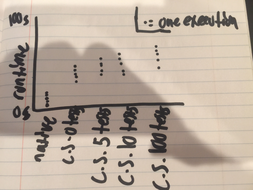
\includegraphics[scale=.75]{images/performance.png}}
        \caption{\emph{This shows the run time difference between the
native program and CrashSimulator in seconds.  Each dot indicates an
        execution.  The X axis shows time values for native executions, and
        executions under CrashSimulator with 0, 5, 10, and 100 tests
        performed respectively.
}}
         \label{figure:performance}

    \end{figure}


{\bf Findings.} Overall, the performance of CrashSimulator is around
an order of magnitude slower than the original program being executed
natively.  It should be noted that in most cases
this slowdown is somewhat mitigated by CrashSimulator's ability to process
tests asynchronously and in other situations it will be more efficient than
running the program natively since {\tt rr's} replay does not require
actual execution of most system calls.  This means that CrashSimulator
avoids the system call overheads, such as I/O.
Even without these improvements, however, CrashSimulator's runtime is more
than manageable when the value it provides is taken into account.  The
cumulative runtime required to execute the tests required to find the QQQ
bugs listed in Table~\ref{table:unexpectedtypes} is around HHHH minutes.
Given this success, the increased runtime is worth the wait.

\section{Related Work}
\label{SEC:related-work}

In constructing SEA and CrashSimulator, we examined a number of previous
studies in bug detection, data mining, environmental influence on
application behavior, and protocols for checking program responses to anomalous
situations. This section
summarizes a few earlier initiatives in each of these areas and discusses
their relevance to the development of our tool.

% One of the major limitations of many automated testing tools is a reliance
% on the availability of a target application's source code.  Out of the top
% XXX automated testing tools (as ranked by YYYY), ZZZZ have this
% dependency.\preston{cite} While open source software has dramatically
% increased in popularity over recent years, closed source dependencies are
% still a major concern.\preston{cite}  Any tool that requires access to
% source code will have diminished capability in projects incorporating
% closed source components.


\iffalse
While there is a vast amount of literature on test
generation~\cite{ammann2008introduction, mcminn2004search,
  puasuareanu2009survey, dias2007survey}, much less work
has focused on issues of portability, and tests of whether software
behaves consistently in different environments.  Prior work on
CheckAPI~\cite{rasley2015detecting} and
NetCheck~\cite{Zhuang_NSDI_2014} begins to fill this gap and this paper
builds upon those results.
%
%\paragraph{Detecting Environmental Bugs.}
%
%NetCheck; CheckAPI; stub injection; detecting machine specific bugs
%(e.g. numeric/memory limitations); testing error handlers; \dots


Crash reproduction by test case mutation~\cite{DBLP:conf/sigsoft/XuanXM15}.

\fi


\noindent
{\bf Static analysis. }
\label{rel-static-analysis}
Tools based on static analysis techniques, such as abstract interpretation,
model checking, and symbolic execution, have been successfully
used to
detect bugs resulting from incorrect API usage. Examples of these tools
include
SLAM~\cite{Ball_adecade, Ball:2002:SLP:503272.503274} and, more recently,
CORRAL~\cite{DBLP:conf/sigsoft/LalQ14} for conformance checking of Windows
device drivers against the Windows kernel API,
FindBugs~\cite{DBLP:conf/oopsla/HovemeyerP04} for detecting API usage bugs
in Java programs, FiSC~\cite{Musuvathi04modelchecking} for finding bugs in
TCP implementations, and the Explode
system~\cite{Yang:2006:ELG:1298455.1298469} for detecting crash recovery
bugs in file system implementations.  Likewise, INFER has found success at
Facebook in analyzing units of code as they are
committed~\cite{INFERFacebook}. Unlike CrashSimulator, these
approaches depend on the availability of source or byte code.

Static analysis techniques have also been
used to detect portability issues related to what happens when an
application encounters different
versions of the external components on which
it depends~\cite{silakov2010improving, javacompliance-www}. Like
CrashSimulator, these techniques
address the application's interactions with its
environment. However, these studies were focused on proving that the
environments behaved as expected.
CrashSimulator is only interested in the application's
response to anomalies.

\iffalse
\noindent
{\bf Specification and run-time verification.}
Substantial work has been done in validating API and protocol behaviors,
e.g., finding faults in the Linux TCP implementation, SSH2 and
RCP~\cite{Udrea:2008}, BGP configuration~\cite{Feamster:2005}, and
identifying network vulnerabilities~\cite{ritchey-sp00}.
\fi

\noindent
{\bf API protocol mining.}
Extensive work has been done on mining source code to learn API protocols
and use them to detect common usage violations, such as missing method calls
(see, e.g.,~\cite{mariani2007compatibility,
DBLP:journals/ase/WasylkowskiZ11, DBLP:conf/icse/PradelJAG12,
DBLP:journals/tosem/MonperrusM13, DBLP:conf/icse/JamrozikSZ16}). These
techniques primarily target object component interactions, rather than
system calls to generate test suites. However, the techniques explored in
these works could be used to mine system call patterns in source code.
This will enable researchers
to find checkers that identify incorrect responses to environmental
anomalies. So far, we have specified these checkers manually for
CrashSimulator.  Data mining techniques could be adapted in the years
ahead to reduce the manual effort required.

\noindent
{\bf Tracing and log mining.}
Similar to API protocol mining, substantive work has been done using
log files to detect anomalies~\cite{pinpoint,
jiang_abnormal_trace_detection_icac_2005, xu2009detecting, lou2010mining2}
and to aid in program understanding~\cite{yuan2010sherlog,
beschastnikh_synoptic_fse_2011, csight_icse_2014}.
For example, CheckAPI~\cite{rasley2015detecting}
and NetCheck~\cite{Zhuang_NSDI_2014} both
use system call traces to diagnose an application's violations of
cross-platform portability.  CrashSimulator in some ways takes these
techniques a step further by using
system call traces
to test responses to known environmental anomalies.
This more active approach can expose bugs that
are invisible to passive log mining.


\noindent
{\bf Environmental Influence and Cross-Platform Portability.}
Negotiating the influence of the environment in which an
application is deployed has been investigated from several
perspectives. One approach, referred to previously,
is to build ``portable'' systems
that have cross-platform capabilities.
Using wrapper subroutines
can enable cross-platform portability
of APIs~\cite{bartolomeicompliance} through system call delegation.
These wrappers can be automatically generated through techniques like
system call interposition ~\cite{Guo:2011:CUS:2002181.2002202}, a
technique that can also be used to detect and prevent security
violations~\cite{Hofmeyr:1998:IDU:1298081.1298084,
Acharya:2000:MUP:1251306.1251307}.
Other works that target complementary classes of portability problems
include the detection of configuration-related bugs~\cite{skoll:icse:2004,
Yilmaz:issta:2004, Fouche:issta:2009, Kastner12, Nguyen14} and
cross-browser incompatibilities for web
applications~\cite{DBLP:conf/icsm/ChoudharyVO10, silakov2010improving,
DBLP:conf/icse/Choudhary11, Mesbah:2011:ACC:1985793.1985870,
DBLP:conf/icst/DallmeierP0MZ14}.  Static analysis tools, such as those
mentioned earlier in this section, have also been applied to
detection of differences between versions of external components.

Such studies have helped to define the influence of an environment on
applications and thus provide a background to our work.  Our tool applies
these fundamental ideas to testing an application's response to anomalies.

\noindent
{\bf Testing exception handling and conformance.}
A few researchers have developed testing techniques aimed at checking
whether programs respond appropriately to anomalous situations.  For
example, Fu et al. introduced data flow testing techniques that require
tests from the points at which exceptions are thrown to the points
at which they are handled in Java code. The purpose is to discover whether
programs respond correctly to exceptional situations anticipated by the
programmer~\cite{DBLP:journals/tse/FuMRW05}.  Koopman and DeVale developed
a system to detect bugs in error handling code related to calls to POSIX
functions~\cite{Koopman00theexception}.  Miller et al. cover the kernel as
a source of unexpected program inputs and test applications by simulating
them~\cite{murphyslaw}.
Other approaches to conformance checking of POSIX operations use model
based testing~\cite{Dadeau:2008:CSM:1433121.1433137,Farchi02}.

Unlike these approaches, CrashSimulator does not exclusively target error
handling code or anomalies that only involve individual system calls.
Additionally, it focuses on collecting and simulating
problematic features of specific
deployment environments.
That said, such testing techniques
can help identify additional anomalies  to add to our repository.

{\bf Smart Fuzzing.}
Smart fuzzers monitor and guide executions to
trigger code paths that are unlikely to be reached
otherwise~\cite{smartfuzzing, taintbasedfuzzing}.
At this point, they make a binary decision about
whether the application correctly handled the input or not.
Typically, a determining factor will be an actual crash by the application.
This is similar to SEA's use of checkers to decide whether
to accept or reject a given test
execution, based on whether or not it observed a specific system call behavior.
In both cases, the tools can demonstrate whether a given code path handles a
situation correctly, but cannot prove that the code path is robust against
other problematic inputs.  In the future, CrashSimulator could use smart
fuzzing path exploration techniques to generate tests that reach relevant
system calls and apply SEA at that point.

%\noindent
%{\bf Runtime verification:}
%Runtime verification (RV)
%techniques~\cite{DBLP:conf/rv/2010, Liu:2007:WCC:1973430.1973449, Lu_ASPLOS_2006,
%Archer:2007:ICT:1236360.1236382, Verbowski_OSDI_2006, Tucek_SOSP_2007,
%Park_ASPLOS_2009,DBLP:journals/jlp/LeuckerS09}
%can detect violations of properties on specific executions
%but do not show that the software satisfies the specification for every
%possible input or on every possible execution.
%Many of these techniques find general violations of
%properties, such as atomicity~\cite{Park_ASPLOS_2009, Verbowski_OSDI_2006}.
%Other RV techniques enable checking program-specific requirements
%usually specified with formal languages, such as automata or logic
%formalisms~\cite{DBLP:conf/vmcai/BarringerGHS04, DBLP:conf/kbse/GiannakopoulouH01}.
%
%Many RV approaches instrument code to capture relevant
%events or application state and insert executable
%assertions~\cite{Orso:2002:GSC:566172.566182, DBLP:conf/icse/ClauseO11,
%DBLP:books/sp/Liblit2007, Jin:2010:ISS:1932682.1869481, Barnett01spyingon,
%DBLP:journals/jss/BarnettS03}.
%However, inserting pre- and post-conditions obscures the fact that the
%specification can be treated as a parallel construct to the
%implementation~\cite{Barnett01spyingon, DBLP:journals/jss/BarnettS03}.
%Instead, an architecture can be used for runtime verification of .NET
%components by running the model and the implementation side-by-side,
%comparing results at method boundaries~\cite{Barnett01spyingon,
%DBLP:journals/jss/BarnettS03}.
%CheckAPI does not require application instrumentation, assuming a tracing
%mechanism exists in the API~\cite{strace, Cappos_CCS_10}.

%Like CheckAPI,
%several other (runtime and static) checking techniques
%allow the use of languages more familiar to
%programmers.
%The WiDS checker allows using a scripting language to specify properties of a
%distributed system~\cite{Liu:2007:WCC:1973430.1973449}.
%Contracts written in a C-like language can specify components for use
%in TinyOS applications~\cite{Archer:2007:ICT:1236360.1236382}.
%CheckAPI allows
%programmers to choose the language for PSI construction or simply to
%use an existing implementation. Lastly, work on deterministic
%replay~\cite{Viennot13} enables record-replay techniques on multi-core
%systems and could help improve CheckAPI-MT performance.


\iffalse
\noindent
{\bf Application-specific fault detection.}
Pip~\cite{reynolds2006pip} and Coctail~\cite{xue2012using} are distributed
frameworks that enable developers to construct application-specific models,
which have proven effective at finding detailed application flaws. However,
utilizing these methods requires a knowledge of what failure needs must
be acquired, and a specification of all relevant system properties. 
NetCheck diagnoses application failures without application-specific
models.  Khanna~\cite{khanna2007automated} identifies the source of
failures using a rule base of allowed state transition paths.
%However, it requires specialized human-generated rules for each
%application.
CrashSimulator leverages NetCheck's approach to simulate identified
anomalies in network behavior, file system behavior, and other environmental-specific conditions. This enables the tool to test
applications other than the ones with which the anomalies were originally
discovered.
\fi


%% The following is old stuff -- not sure how much should be integrated
%% into the above.
\begin{comment}
\subsection{Existing Techniques}

Existing tools can be roughly divided into two categories, black-box
and white-box, based on the techniques they use to perform their
testing. Black-box tools simply manipulate the inputs of the
application under test and observe the resultant outputs. White-box
tools, on the other hand, perform complex analysis of the application's
source code in order to reason about what inputs are likely to produce
interesting outputs. Each of these methodologies have their own
advantages and disadvantages.

White-box testing tools typically rely on a similar set of techniques,
including constraint solving of branch statements in an application's
code and symbolic execution of an application's code in order to
generate inputs that optimally exercise the application's code paths.
These techniques, while powerful, are not without their downsides.
First, both techniques are computationally-expensive. Furthermore,
symbolic execution can not always accurately represent actual execution,
and so there may be deviations in results. Similarly, it is difficult to efficiently
solve a series of constraints in order to exercise a particular code.
In many
circumstances, a given set of
generated inputs can exercise an intended code path  due to external dependencies that the tool cannot
analyze. For example, a white-box testing tool cannot reliably generate
inputs that are guaranteed to exercise a code path if they rely on the availability of an
operating system resource.  Finally, white-box tools
typically require that an application's source code be available, which
is not always the case. Even advanced white-box tools that analyze machine code can be stymied in situations where an
application's executable has been packed or encrypted.

The alternative, black-box tools, have their own set of issues. They do
not have an understanding of what an application is actually doing
during execution, which means they are only able to submit inputs and
observe outputs.  The upside of this technique is simplicity. Black-box
tools do not need to understand and analyze an
application's code, which reduces their complexity immensely. Also,
their testing process, mutating inputs and observing outputs, is
computationally inexpensive. The downside of this simplicity is that they
cannot craft inputs with any sort of intelligence. This means that a
great deal of time can be spent mutating inputs without much success in
terms of bug identification. Also, they cannot specifically identify 
the source of faults in an application. They can only signal that a
fault has occurred at some point during a test run.  Furthermore, like
white-box tools, these tools fail to take into account the environment
in which the application is running.  \subsection{White-box Tools}

White-box testing has been an area of intense interest in recent
writing. Microsoft's SAGE and Bell Labs' DART are two examples of
such tools that take different approaches to the same overall
white-box technique.

\subsubsection{DART}

DART is a white-box testing tool that supports testing of
applications written in the C programming language. It is
capable of generating a test harness for an application's
functions by through static analysis of the application's
source code. This harness is then used for two phases of
testing. First, it performs random testing and observes the
application's behavior. Based on this random testing and
symbolic execution of the application's source code, DART
generates a series of inputs that will be used in the second
phase of testing.  These inputs are designed to direct the
application down specific execution paths, observing the
programs behavior and reporting faults as they are identified.
DART operates on the assumption that the functions being
evaluated have no side-effects and that the application is able
to interact appropriately with its environment.  More
information can be found in \textbf{\emph{PAPER TITLE HERE}}

\subsubsection{SAGE}

SAGE differs from many other white-box testing tools in that it
analyzes a compiled application's machine code rather than the
application's uncompiled source code. This allows SAGE to
operate on applications that were compiled from a variety of
programming languages. It first runs the application under test
with a set of well formed inputs and records an
instruction-level trace of the application's execution. Next,
it analyzes this trace in order to identify constraints that
guard different paths of execution. SAGE then solves these
constraints and, based on these solutions, generates inputs
that are able to exercise specific paths of execution.

\subsection{Black-box tools}


\subsection{Trace Analysis Tools}

Much of CrashSimulator's work on system call trace analysis is
based on previous work on NetCheck and CheckAPI

\subsubsection{NetCheck}

This implementation of CrashSimulator relies of NetCheck for
system call trace analysis. NetCheck uses two strategies to
identify potential fault areas from system call trace. The
first is a model based simulation of the system calls relevant
to network communication from the input trace. System calls are
organized according to a POSIX socket API dependency graph and
prioritized based on the order in which the system calls should
be made in an ideal scenario.  For example, a client
application should not be making a \emph{connect} system call
before it has set up its socket with the appropriate
\emph{socket} system call.  The model assumes that all system
calls are atomic and that they cannot happen simultaneously.
This allows a definite global order to be created.

Once a global ordering is in place each system call is
evaluated based on the previous system calls. Return values and
parameters passed in are taken into account. If the system call
is feasible it is accepted and the next system call is
evaluated. If the system call is not feasible given the current
system call context it is rejected and logged. In addition,
system calls that return a value indicating some sort of
network failure are recorded. After all system calls have been
evaluated a NetCheck attempts to diagnose the source of any
errors encountered. It is this diagnosis that CrashSimulator
uses when deciding where and how to mutate the ``ideal run''
system call trace it is operating on.

\subsubsection{CheckAPI}

% TODO: Expand this
\textbf{\emph{This needs to be expanded}}
CheckAPI attempts to identify
\end{comment}

\section{Conclusion}
\label{SEC:conclusion}

When an application fails upon deployment,
the cause could likely be the result
of unexpected interactions between
an application and its environment.  Although finding and eliminating
faults in applications is a key concern for software developers, it is
impractical to run actual tests  of an application in every possible
environment in
which it could be deployed.  To address this problem, we introduced
CrashSimulator, a strategy and tool
that can determine whether an application will
respond correctly to anomalous environmental conditions.

The tool records system call traces from the application under test,
mutates return values and/or program state to simulate execution in the
anomalous environment, and uses sub- sequent system calls to decide whether
a correct or incorrect response as occurred. This allows CrashSimulator to
test an application running in one environment as if it were running in
another. Operating on system calls gives the tool  a ``universal'' way to
encode and inject anomalies. Consequently, a set of mutations can be
collected from any existing application for use in testing other new or
existing applications. In this way, an ever-expanding ``test suite'' can be
created, allowing lessons learned from bugs in one application to benefit
many others.

Our evaluation of CrashSimulator has shown it to be both usable and
effective.  In our survey of developers, CrashSimulator compared favorably
against both AFL and Mutiny across self-reported developer skill levels.
CrashSimulator was particularly favored by developers with more operating
systems experience, but even developers with low OS experience were pleased
with its ability to let them find bugs by taking advantage of
the expert knowledge encoded in the tool.
In our user study, a total of
19 new bugs were identified in popular applications.
These bugs have been reported to the
affected parties and 5 have already been corrected.

%  CrashSimulator was able to identify bugs related to unusual
%  file types in 15 applications and bugs related to slow network performance
%  in 10 network applications and libraries.  Additionally CrashSimulator
%  found filesystem related bugs in 6 applications and libraries with
%  facilities for moving files within a system's filesystem.  The low overhead
%  introduced by CrashSimulator's technique meant that it was able to find
%  these bugs quickly in spite of its unoptimized implementation.

In the long term, we
envision a public repository of anomalies along with CrashSimulator test
patterns that can be applied to new or existing applications.
In addition to expanding the repository of anomalies, as well as exploring
opportunities to further automate the discovery process, we plan on improving
CrashSimulator in two different directions.  First, we plan in improving
CrashSimulator's bug detection capabilities by analyzing application's attempts
to recover from the anomalies to which we have exposed them.  This would allow
us to make determinations about whether an application is correctly recovering
from an error rather.  Second, we hope to improve CrashSimulator so that it can
understand and mutate common data formats.  This would allow CrashSimulator
to fuzz test data processing code while taking advantage of its
replay-based architecture to avoid re-executing portions of the application
uninvolved in testing.


\bibliographystyle{IEEEtran}
\bibliography{IEEEabrv,bibdata}

\end{document}
